%%%%%%%%%%%%%%%%%%%%%%%%%%%%%%%%%%%%%%%%%%%%%%%%%%%%%%%
%% Modelo LaTeX de monografia UCS                    %%
%% Data de Modificação: 10 de agosto de 2021         %%
%%                                                   %%
%%%%%%%%%%%%%%%%%%%%%%%%%%%%%%%%%%%%%%%%%%%%%%%%%%%%%%%

% ---
\documentclass[
	12pt,				% tamanho da fonte
	openright,			% capítulos começam em pág ímpar (insere página vazia caso preciso)
	oneside,			% para impressão em uma folha. Oposto a twoside
	a4paper,			% tamanho do papel. 
	% -- opções do pacote babel --
	english,			% idioma adicional para hifenização
	french,				% idioma adicional para hifenização
	spanish,			% idioma adicional para hifenização
	brazil				% o último idioma é o principal do documento
	]{abntex2}

% ---
% Pacotes básicos 
% ---
\usepackage[table]{xcolor}
\usepackage{adjustbox}
\usepackage{amsmath}
\usepackage{chemformula} 
\usepackage{chemfig} 
\usepackage{mathtools}
\usepackage[printonlyused]{acronym}

\usepackage{setspace}

\usepackage{times}
\usepackage[T1]{fontenc}		% Seleção de codigos de fonte.
\usepackage[utf8]{inputenc}		% Codificação do documento (conversão automática dos acentos)
\usepackage{lastpage}			% Usado pela Ficha catalográfica
\usepackage{indentfirst}		% Indenta o primeiro parágrafo de cada seção.
\usepackage{color}				% Controle das cores
\usepackage{graphicx}			% Inclusão de gráficos
\usepackage{subcaption}
\usepackage{ragged2e}
%\usepackage{microtype} 			% para melhorias de justificação

\usepackage[alf,
            versalete,
            abnt-emphasize = bf,                % destaca o titulo em negrito;
            abnt-etal-list = 3,                 % trabalhos com mais de 3 autores recebem et al.,;
            abnt-etal-text = it,                % escreve o et al., em itálico;
            abnt-and-type = e,                 % usa o caractere 'e' para mais de um autor;
            abnt-last-names = abnt,             % trata sobrenomes 'estritamente' conforme a ABNT; e
            abnt-repeated-author-omit = yes     % autores com + de uma entrada recebem '____.'
]{abntex2cite}

% pacotes de tabelas
\usepackage{multicol}	% Suporte a mesclagens em colunas
\usepackage{multirow}	% Suporte a mesclagens em linhas
\usepackage{longtable}	% Tabelas com várias páginas
\usepackage{fr-longtable, ltcaption}% permitir adicionar conclusão na última página de longtable
\usepackage{threeparttablex}    % notas no longtable
\renewcommand\tabularxcolumn[1]{m{#1}} % for vertical centering text in X column
\usepackage{array}

\usepackage{listings}
\usepackage{hyperref}

\AtBeginDocument{% the counter is defined later
  \counterwithout{lstlisting}{chapter}%
}
\makeatletter
\renewcommand{\l@lstlisting}[2]{%
  \@dottedtocline{1}{0em}{1.5em}{\lstlistingname\ #1}{#2}%
}

\renewcommand{\lstlistingname}{Algoritmo}% Listing -> Algorithm
\renewcommand{\lstlistlistingname}{LISTA DE ALGORITMOS}% List of Listings -> List of Algorithms

\usepackage{pgfplots} %graficos
\usepackage{booktabs,makecell}
\usepackage{siunitx}

\usepackage{array}

\usepackage{todonotes}

\usepackage{booktabs}
\usepackage{graphicx}
\usepackage{tabularx}

\setlength{\marginparwidth}{2cm}

\newcolumntype{L}[1]{>{\raggedright\let\newline\\\arraybackslash\hspace{0pt}}m{#1}}
\newcolumntype{C}[1]{>{\centering\let\newline\\\arraybackslash\hspace{0pt}}m{#1}}
\newcolumntype{R}[1]{>{\raggedleft\let\newline\\\arraybackslash\hspace{0pt}}m{#1}}

%=======================================================================
% CONFIGURAÇÕES DE PACOTES
%=======================================================================
\DeclareMathOperator*{\maxi}{Maximizar}
\DeclareMathOperator*{\mini}{Minimizar }

\newcommand{\icol}[1]{% inline column vector
  \left(\begin{smallmatrix}#1\end{smallmatrix}\right)%
}

%------
% Configurações dos Algoritmos/Código
%------
\lstset{language=C,                 % linguagem padrão (pode ser modificada em cada algoritmo/código)   
        basicstyle=\footnotesize,   % tamanho da fonte utilizado para o código
        numbers=left,               % onde colocar os números da linha
        numberstyle=\footnotesize,  %estilo a ser utilizado pelos números
        frame=single                % adiciona um quadro ao redor do código
} 

%=======================================================================
% Informações de dados para CAPA, FOLHA DE ROSTO e FOLHA DE APROVAÇÃO
%=======================================================================
\titulo{Aerochord: Um Hiperinstrumento Musical Controlado por Gestos}
\autor{Rafael Basso Sberse}
\local{Caxias do Sul}
\data{2025}
\orientador{Prof. Dra. Elisa Boff}
% \coorientador{Prof. Dr. Nome do Co-orientador}
\universidade{UNIVERSIDADE DE CAXIAS DO SUL}
\area{ÁREA DO CONHECIMENTO DE CIÊNCIAS EXATAS E ENGENHARIAS}
\preambulo{Trabalho de Conclusão de Curso apresentado como requisito parcial à obtenção do título de Bacharel em Ciência da Computação na Área do Conhecimento de Ciências Exatas e Engenharias da Universidade de Caxias do Sul.}
\tipotrabalho{Projeto de Diplomação}
% ---

% alterando o aspecto da cor azul
\definecolor{blue}{RGB}{41,5,195}

% informações do PDF
\makeatletter
\hypersetup{
     	%pagebackref=true,
		pdftitle={\@title}, 
		pdfauthor={\@author},
    	pdfsubject={\imprimirpreambulo},
	    pdfcreator={LaTeX with abnTeX2},
		pdfkeywords={abnt}{latex}{abntex}{abntex2}{trabalho acadêmico}, 
		colorlinks=true,       		% false: boxed links; true: colored links
    	linkcolor=black,          	% color of internal links
    	citecolor=black,        	% color of links to bibliography
    	filecolor=magenta,      	% color of file links
		urlcolor=black,
		bookmarksdepth=4
}
\makeatother
% --- 

% ---
% Posiciona figuras e tabelas no topo da página quando adicionadas sozinhas
% em um página em branco. Ver https://github.com/abntex/abntex2/issues/170
\makeatletter
\setlength{\@fptop}{5pt} % Set distance from top of page to first float
\makeatother
% ---

% ---% Possibilita criação de Quadros e Lista de quadros.
% Ver https://github.com/abntex/abntex2/issues/176
%
\newcommand{\quadroname}{Quadro}
\newcommand{\listofquadrosname}{Lista de quadros}

\newfloat[chapter]{quadro}{loq}{\quadroname}
\newlistof{listofquadros}{loq}{\listofquadrosname}
\newlistentry{quadro}{loq}{0}

% configurações para atender às regras da ABNT
\setfloatadjustment{quadro}{\centering}
\counterwithout{quadro}{chapter}
\renewcommand{\cftquadroname}{\quadroname\space} 
\renewcommand*{\cftquadroaftersnum}{\hfill--\hfill}

\setfloatlocations{quadro}{hbtp} % Ver https://github.com/abntex/abntex2/issues/176
% --- 
% Espaçamentos entre linhas e parágrafos 
% --- 

% O tamanho do parágrafo é dado por:
\setlength{\parindent}{1.3cm}

% Controle do espaçamento entre um parágrafo e outro:
\setlength{\parskip}{0.2cm}  % tente também \onelineskip

% ---
% compila o índice
% ---
\makeindex
% ---

% ----
% Início do documento
% ----
\pgfplotsset{compat=1.15}
\begin{document}

% Seleciona o idioma do documento (conforme pacotes do babel)
\selectlanguage{brazil}

% Retira espaço extra obsoleto entre as frases.
\frenchspacing 

%=======================================================================
% ELEMENTOS PRÉ-TEXTUAIS
%=======================================================================

% ----------------------------------------------------------------------
% Capa
% ----------------------------------------------------------------------
\imprimircapa

% ----------------------------------------------------------------------
% Folha de rosto
% ----------------------------------------------------------------------
\imprimirfolhaderosto

% ----------------------------------------------------------------------
% Folha de aprovação
% ----------------------------------------------------------------------
\newpage
% Isto é um exemplo de Folha de aprovação, elemento obrigatório da NBR
% 14724/2011 (seção 4.2.1.3). Você pode utilizar este modelo até a aprovação
% do trabalho. Após isso, você pode substituir todo o conteúdo deste arquivo por uma
% imagem da página assinada pela banca com o comando abaixo:
%
% \includepdf{folhadeaprovacao_final.pdf}
%
\begin{folhadeaprovacao}

	\begin{center}
    	{\ABNTEXchapterfont\bfseries\large\MakeUppercase\imprimirautor}
		
    	\vspace*{\fill}\vspace*{\fill}
    	\begin{center}
 	\ABNTEXchapterfont\bfseries\large\MakeUppercase\imprimirtitulo
   	\end{center}
    	\vspace*{\fill}
    	
    	\hspace{.45\textwidth}
    		\begin{minipage}{.5\textwidth}
    		\ABNTEXchapterfont\large\imprimirpreambulo
        		~\\
        		~\\
        		~\\
    		\end{minipage}%
    	\vspace*{\fill}
   	\end{center}
   
   	\ABNTEXchapterfont\bfseries\large\MakeUppercase{Banca Examinadora}
    
    \normalfont
   
   \assinatura{\ABNTEXchapterfont\large\imprimirorientador \\ Universidade de Caxias do Sul - UCS}
 
    %¨Altere os dados dos membros da banca
  
   \assinatura{\ABNTEXchapterfont\large{Prof. Dr. Marcelo Luís Fardo} \\ Universidade de Caxias do Sul - UCS}
   
   \assinatura{\ABNTEXchapterfont\large{Prof. Dr. Marcos Eduardo Casa} \\ Universidade de Caxias do Sul - UCS}
   
\end{folhadeaprovacao}

% ----------------------------------------------------------------------
% Dedicatória (opcional).
% ----------------------------------------------------------------------
%\imprimirdedicatoria{1-pre-textuais/dedicatoria}

% ----------------------------------------------------------------------
% Agradecimentos (opcional).
% ----------------------------------------------------------------------
% \imprimiragradecimentos{1-pre-textuais/agradecimentos}

% ----------------------------------------------------------------------
% Epígrafe (opcional).
% ----------------------------------------------------------------------
% \begin{epigrafe}
    \vspace*{\fill}
	\begin{flushright}
		\textit{``Não morre aquele que deixou na terra a melodia de seu cântico na música de seus versos.'' \\ 
		\textbf{Cora Coralina}  }
	\end{flushright}
\end{epigrafe}


% ----------------------------------------------------------------------
% Resumo  
% ----------------------------------------------------------------------
\setlength{\absparsep}{18pt}

\begin{resumo}[RESUMO]
Este trabalho propõe a arquitetura e o plano de implementação de um hiperinstrumento musical gestual denominado Aerochord, que utiliza visão computacional por câmera RGB comum para gerar eventos MIDI 2.0 com resolução estendida, buscando democratizar a expressão musical para usuários sem formação técnica em instrumentos e pessoas com mobilidade reduzida. Inicialmente, foi realizada a revisão bibliográfica em interação humano-computador e computação musical, seguida de análise crítica do estado da arte em interfaces gestuais, o que evidencia a lacuna entre acessibilidade, latência e expressividade profissional. Com base nessa investigação, foram definidos os requisitos funcionais e não funcionais para o Aerochord, incluindo processamento de vídeo em tempo real, detecção de pontos de referência das mãos via técnicas de visão computacional, mapeamentos gesto–som preliminares e comunicação via MIDI 2.0 com plano de contingência para modo legado. Foi proposta uma arquitetura modular em C++ em conjunto com o \textit{framework} JUCE, organizada em pipelines buscando minimizar o \textit{jitter}, uso de filas sem bloqueio, \textit{handshake} por \textit{MIDI Capability Inquiry} e inserção de \textit{timestamps} em pacotes universais, de modo a garantir resposta sonora coerente a gestos do performer. Planeja-se, na fase seguinte, avaliação experimental com medições objetivas de latência e precisão de reconhecimento, além de métodos subjetivos de usabilidade e carga cognitiva, incorporando cuidados de privacidade e adaptabilidade a diferentes perfis de usuário e cenários de uso. Esta etapa conceitual estabelece fundamentos robustos para a implementação do protótipo, oferecendo diretrizes técnicas e metodológicas para prototipagem em tempo real e testes experimentais. Espera-se que o Aerochord contribua para o campo de interação humano-computador e computação musical ao apresentar um modelo de hiperinstrumento acessível, responsivo e expressivo, servindo de base para pesquisas futuras em mapeamentos adaptativos e ambientes imersivos.

\textbf{Palavras-chave}: interfaces gestuais, computação musical, MIDI 2.0, democratização musical, visão computacional, hiperinstrumentos, acessibilidade, baixa latência.
\end{resumo}

% ----------------------------------------------------------------------
% Abstract 
% ----------------------------------------------------------------------
% Resumo em Língua Inglesa
\setlength{\absparsep}{18pt}
\begin{resumo}[ABSTRACT]
 \begin{otherlanguage*}{english}

This work presents the development and evaluation of a gestural musical hyperinstrument named Aerochord, which utilizes computer vision with a standard RGB camera to generate MIDI 2.0 events with extended resolution, aiming to democratize musical expression for users without technical training on instruments and for people with reduced mobility. Initially, a literature review was conducted on human-computer interaction and computer music, followed by a critical analysis of the state of the art in gestural interfaces, which highlighted a gap between accessibility, latency, and professional-level expressivity. Based on this investigation, the functional and non-functional requirements for Aerochord were defined, including real-time video processing, hand landmark detection via computer vision techniques, gesture-to-sound mappings, and communication via MIDI 2.0 with a contingency plan for legacy mode. A modular architecture in C++ using the JUCE framework was implemented, organized into pipelines that minimize jitter, utilizing lock-free queues, handshaking via MIDI Capability Inquiry, and the packaging of commands into Universal MIDI Packets to ensure a coherent sonic response to the performer's gestures. The experimental evaluation carried out demonstrated end-to-end latency consistently below the perceptible threshold of 30 ms (95th percentile of 24.45 ms) and low resource consumption, alongside a pilot usability test that evidenced a low entry barrier for users without musical training. The results confirm the technical and practical feasibility of the proposal, establishing a foundation for future developments in polyphony, adaptive mappings, and immersive environments. It is expected that Aerochord will contribute to the fields of human-computer interaction and computer music by presenting a model of an accessible, responsive, and expressive hyperinstrument.


% Coloque após os ":"  as palavras-chave com a primeira 
% letra de cada palavra em maiúscula e separadas por ponto.
\textbf{Keywords}: gesture interfaces, musical computing, MIDI 2.0, musical democratization, computer vision, hyperinstruments, accessibility, low latency.
 \end{otherlanguage*}
\end{resumo}

% ----------------------------------------------------------------------
% Lista de Figuras (se necessário)
% ----------------------------------------------------------------------
% \pdfbookmark[0]{\listfigurename}{lof}
% \listoffigures*
% \cleardoublepage

% ----------------------------------------------------------------------
% Lista de Tabelas (se necessário)
% ----------------------------------------------------------------------
% \pdfbookmark[0]{\listtablename}{lot}
% \listoftables*
% \cleardoublepage

% ----------------------------------------------------------------------
% Lista de Quadros (se necessário)
% ----------------------------------------------------------------------
% \pdfbookmark[0]{\listofquadrosname}{loq}
% \listofquadros*
% \cleardoublepage

% ----------------------------------------------------------------------
% Lista de Algoritmos (se necessário)
% ----------------------------------------------------------------------
% \newlistof{lstlistoflistings}{lol}{\lstlistlistingname}
% \lstlistoflistings*
% \cleardoublepage

% ----------------------------------------------------------------------
% Lista de abreviaturas e siglas (opcional)
% ----------------------------------------------------------------------
\begin{siglas}

\item [IHC]
\begin{acronym}[ABNT]
Interação Humano-Computador
\end{acronym}

\item [IMD]
\begin{acronym}[ABNT]
Instrumento Musical Digital
\end{acronym}

\item [MIDI]
\begin{acronym}[ABNT]
\textit{Musical Instrument Digital Interface}
\end{acronym}

\item [UMP]
\begin{acronym}[ABNT]
\textit{Universal MIDI Packet}
\end{acronym}

\item [MPE]
\begin{acronym}[ABNT]
\textit{MIDI Polyphonic Expression}
\end{acronym}

\end{siglas}


% ----------------------------------------------------------------------
% Lista de símbolos (opcional)
% ----------------------------------------------------------------------
% \include{1-pre-textuais/simbolos}

% ----------------------------------------------------------------------
% Sumário
% ----------------------------------------------------------------------
\pdfbookmark[0]{\contentsname}{toc}
\tableofcontents*
\cleardoublepage

%=======================================================================
% ELEMENTOS TEXTUAIS
%=======================================================================
\textual

\chapter{Introdução}
\label{chap:introducao}

Nas últimas décadas, a interação humano-computador tem-se orientado cada vez mais para interfaces que ofereçam modos de uso naturais e intuitivos, movendo-se além de paradigmas baseados em teclados e dispositivos apontadores (como o \textit{mouse}) para explorar a entrada gestual e multimodal \cite{preece2023interaction}. Paralelamente, a música digital consolidou-se como campo de investigação e aplicação prática, com o surgimento de Instrumentos Musicais Digitais que possibilitam novas formas de criação e execução musical (\textit{performance}) \cite{Roads1996, Miranda2002}. Nesse contexto, as interfaces gestuais musicais emergem como convergência promissora entre IHC (Interface Humano-Computador) e computação musical, propiciando experiências em que movimentos corporais ou de mãos se traduzem diretamente em eventos sonoros \cite{wanderley2000gestural}. 

Com o avanço de arcabouços de desenvolvimento (\textit{frameworks}\footnote{\textit{Frameworks} são conjuntos de bibliotecas e componentes de \textit{software} que fornecem uma base estrutural, abstraindo complexidades de baixo nível para facilitar o desenvolvimento de aplicações.}) acessíveis voltados à visão computacional, como o MediaPipe, e com a disponibilidade de protocolos de alta resolução para controle musical, em especial o padrão MIDI 2.0 (\textit{Musical Instrument Digital Interface}), abre-se a possibilidade de desenvolver sistemas que utilizem equipamentos físicos (\textit{hardware}) comuns. O uso de câmeras de vídeo baseadas no modelo de cores vermelho, verde e azul (\textit{Red, Green, Blue} - RGB) e computadores de uso geral permite, assim, oferecer interações musicais ricas e dinâmicas \cite{lugaresi2019mediapipe,midi_org}.

Ainda que existam diversas propostas acadêmicas e comerciais de interfaces gestuais musicais, persistem barreiras que limitam tanto o acesso quanto a expressividade desses sistemas. Muitas soluções demandam \textit{hardware} especializado e custoso, apresentam latência (tempo de atraso na resposta) que compromete a sensação de fluidez, ou dispõem de resolução de controle insuficiente para atender ao desejo de uma expressão musical rica e detalhada. Além disso, a complexidade técnica inerente a essas interfaces pode afastar usuários sem formação musical ou sem experiência em tecnologias avançadas. Indivíduos com mobilidade reduzida frequentemente enfrentam dificuldades adicionais ao operar instrumentos convencionais ou mesmo soluções digitais que requerem motricidade fina. Diante desse panorama, revela-se a lacuna principal que orientou este trabalho: a necessidade de conceber um hiperinstrumento musical gestual que, apoiado em visão computacional por câmeras de vídeo de uso comum (\textit{webcams}) e adotando o protocolo MIDI 2.0, fosse simultaneamente acessível, de baixa latência e capaz de oferecer expressividade profissional.

O objetivo geral deste trabalho consistiu em desenvolver e avaliar um hiperinstrumento denominado Aerochord, que utiliza controle gestual via câmera RGB para geração de eventos MIDI 2.0 com resolução estendida, de modo a democratizar a expressão musical e atender a usuários sem treinamento formal. Para tanto, o projeto cumpriu os seguintes objetivos específicos: revisou o estado da arte em interfaces musicais gestuais, identificando paradigmas de interação, tecnologias de captura e lacunas existentes; especificou requisitos funcionais e não funcionais para o Aerochord, enfatizando acessibilidade, latência e expressividade; definiu e implementou uma arquitetura modular de programas de computador (\textit{software}), baseada em visão computacional e comunicação via MIDI 2.0, orientada ao desempenho em tempo real; elaborou mapeamentos entre os gestos e os sons que equilibram intuitividade e profundidade expressiva; e executou a validação técnica do sistema por meio de testes de desempenho e medição de latência.

A justificativa para este projeto é multidimensional. Do ponto de vista social, buscou-se ampliar o acesso à criação musical ao oferecer uma alternativa de baixo custo que dispensa dispositivos especializados, favorecendo pessoas sem conhecimento técnico em música e indivíduos com limitações motoras. Do ponto de vista acadêmico e tecnológico, preencheu-se a lacuna identificada no estado da arte por meio da combinação de visão monocular acessível (utilização de uma única lente de câmera), arquitetura de \textit{software} de baixa latência na linguagem C++ em conjunto com o \textit{framework} JUCE, e o uso de MIDI 2.0 para integração com as principais Estações de Trabalho de Áudio Digital (\textit{Digital Audio Workstations} - DAWs\footnote{DAWs são \textit{softwares} ou sistemas completos que permitem gravar, editar, mixar e masterizar áudio digital profissionalmente.}). Essa combinação evidencia inovação ao propor um sistema que une facilidade de uso a requisitos de execução musical de nível profissional. Ademais, o Aerochord insere-se no campo de IHC como um caso de uso prático para técnicas de reconhecimento gestual em tempo real, contribuindo com implementações que podem orientar desenvolvimentos futuros.

Para conduzir esta pesquisa e o subsequente desenvolvimento, adotou-se uma abordagem dividida em três frentes: a revisão bibliográfica para fundamentação teórica em bases como \textit{Google Scholar}, na Conferência Internacional sobre Novas Interfaces para Expressão Musical (\textit{New Interfaces for Musical Expression} - NIME) e na Biblioteca Digital da \textit{Association for Computing Machinery} (ACM); a engenharia de \textit{software}, englobando a implementação estruturada de captura de imagem, processamento de inteligência artificial e geração sonora; e, por fim, a etapa de avaliação experimental, voltada à coleta e análise de métricas de desempenho e tempo de resposta do sistema.

O presente documento está estruturado da seguinte forma: no Capítulo~\ref{cap:interacao_gestual_e_hiperinstrumentos}, apresentam-se os conceitos fundamentais de IHC e hiperinstrumentos que sustentam a proposta; no Capítulo~\ref{cap:computacao_musical}, detalham-se os aspectos de computação musical e o protocolo MIDI, justificando a adoção do MIDI 2.0; o Capítulo~\ref{cap:analise_estado_arte_interfaces_musicais_gestuais} examina criticamente o estado da arte em interfaces gestuais musicais e identifica a lacuna que motiva o Aerochord; o Capítulo~\ref{chap:desenvolvimento_proposta} descreve em detalhes a arquitetura modular desenvolvida e a implementação do mapeamento entre gesto e som; o Capítulo~\ref{chap:testes_resultados} apresenta a metodologia de testes aplicada, juntamente com a análise empírica dos resultados obtidos em termos de latência e estabilidade; por fim, o Capítulo~\ref{chap:consideracoes_finais} conclui o trabalho, sumarizando as contribuições alcançadas, discutindo as limitações encontradas e apontando direções para trabalhos futuros.

Dessa forma, esta introdução orienta o leitor sobre a relevância do tema, o problema enfrentado, os objetivos e a justificativa do Aerochord, bem como o escopo e a estrutura do documento que consolida toda a jornada de pesquisa e desenvolvimento do projeto.
\chapter{Interação Gestual e Hiperinstrumentos}
\label{cap:interacao_gestual_e_hiperinstrumentos}

Neste capítulo, a fundamentação teórica que orientou o projeto (\textit{design}) e os objetivos do Aerochord é aprofundada. Inicialmente, na seção \ref{sec:iteracao_multimodal}, o campo da Interação Humano-Computador (IHC) é explorado, destacando-se o paradigma da interação gestual como uma modalidade de controle expressiva e natural, capaz de resgatar a corporeidade e a nuance da execução musical (\textit{performance}). Em seguida, na seção \ref{sec:dispositivos_e_ferramentas_deteccao_gestos}, são examinadas as principais ferramentas e tecnologias de detecção de gestos, com ênfase em abordagens de visão computacional que fundamentaram a solução técnica adotada no projeto. Por fim, na seção \ref{sec:hiperinstrumentos_musicais} apresenta-se e discute-se o conceito de hiperinstrumento, arcabouço conceitual (\textit{framework}) que define a natureza do instrumento materializado pelo Aerochord: um sistema musical gestual de alta expressividade, acessível e extensível. Assim, é apresentado um panorama organizado das bases teóricas e tecnológicas que sustentam o desenvolvimento do projeto, mostrando como os temas abordados — a interação gestual na IHC, as técnicas de detecção e o conceito de hiperinstrumento — se relacionam para fundamentar a arquitetura da solução.

\section{Interação Multimodal e Gestual}
\label{sec:iteracao_multimodal}

A área de Interação Humano-Computador (IHC) tem como objetivo superar as restrições impostas por interfaces convencionais, como teclado e \textit{mouse} (dispositivo apontador), ao buscar meios de interação mais naturais, intuitivos e centrados nas capacidades humanas. À medida que sistemas computacionais se integram de forma crescente ao cotidiano, surge a demanda por interfaces que reflitam a fluidez e a riqueza da comunicação interpessoal, reduzindo a distância entre a intenção do usuário e a resposta do sistema. Esse contexto justificou a investigação de modalidades gestuais no projeto Aerochord, por se tratar de uma abordagem que aproxima a interação digital dos modos como as pessoas se comunicam entre si \cite{preece2023interaction}.

\subsection{O Paradigma da Interação Multimodal}
\label{subsec:paradigma_iteracao_multimodal}

Sistemas multimodais são aqueles capazes de processar, de maneira coordenada, múltiplas modalidades de entrada, como fala, gestos, olhar e toque, de modo que cada canal contribua para uma interpretação mais precisa da intenção do usuário. Por meio de fusão de sinais e integração temporal e semântica, esses sistemas combinam fluxos sensoriais distintos para aumentar a robustez e a adaptabilidade da interface. Isso permite que falhas ou ambiguidades em um modo sejam compensadas por outro. 

Essa coordenação entre canais também oferece flexibilidade, pois o usuário pode escolher a modalidade mais conveniente conforme o contexto e suas preferências. Além disso, promove maior naturalidade ao refletir padrões típicos da comunicação entre pessoas \cite{oviatt2018multimodal2, oviatt2019multimodal3}. Interfaces multimodais também conseguem se adaptar dinamicamente a mudanças ambientais, alternando ou combinando modos de entrada para manter a eficácia da interação. Esses fatores justificam o estudo aprofundado de modalidades específicas, como a gestual, dentro de um quadro multimodal mais amplo.

A multimodalidade confere vantagens centrais em termos de usabilidade: flexibilidade para o usuário selecionar o canal mais adequado, robustez ao mitigar falhas em uma modalidade por meio de outra, e maior naturalidade ao espelhar padrões comunicativos humanos. Tais benefícios reforçam a importância do estudo de interfaces gestuais, mesmo em projetos que foquem primariamente nessa modalidade, pois elas se inserem num ecossistema de interação que visa experiências mais ricas e resilientes \cite{oviatt2019multimodal3}.

\subsection{A Expressividade da Interação Gestual na Música}
\label{subsec:expressividade_iteracao_gestual}

A interação gestual \textit{mid-air} (gestos realizados no ar) refere-se a movimentos livres de mãos e braços no espaço, sem contato físico com superfícies, proporcionando potencial expressivo elevado, mas impondo desafios ergonômicos, perceptuais e técnicos. Entre esses desafios estão a fadiga muscular decorrente de gestos prolongados, a ausência de retorno (\textit{feedback}) tátil natural, as variações de iluminação e cenário que afetam a detecção, e a necessidade de latência muito baixa para manter a sensação de controle imediato. Além disso, torna-se necessário incorporar \textit{feedback} audiovisual ou háptico (relativo ao tato) artificial para confirmar o reconhecimento dos gestos \cite{aigner2012understanding}. Esses aspectos exigem projetos cuidadosos de detecção, filtragem de ruído e mecanismos de confirmação, de modo a preservar a fluidez e a confiança do usuário na interface gestual.

Contudo, habilitar controle por gestos não é suficiente; é imprescindível que o repertório gestual seja intuitivo e fácil de aprender. Metodologias formais de elicitação de gestos para interação \textit{mid-air} são aplicadas com o objetivo de identificar movimentos que os usuários associam espontaneamente a determinadas ações. Esse raciocínio orientou o mapeamento no Aerochord, garantindo que os gestos implementados coincidissem com expectativas naturais e se mantivessem ergonômicos, evitando movimentos excessivamente amplos ou complexos que pudessem comprometer a experiência \cite{vogiatzidakis2018gesture}.

No contexto musical, gestos e som estão intrinsecamente conectados. Em instrumentos tradicionais, a execução sonora já se baseia em atos gestuais refinados, nos quais movimentos sutis determinam nuances de timbre, dinâmica e articulação. Controlar sistemas digitais por meio de gestos busca resgatar essa corporeidade, permitindo manipulações contínuas e multidimensionais de vários parâmetros sonoros (posição, velocidade, aceleração, trajetória e intensidade) que interfaces convencionais dificilmente capturam com fidelidade. Estudos na área de controle gestual musical mostram que a riqueza e a precisão dos dados capturados influenciam diretamente a expressividade do intérprete, reforçando que a modalidade gestual é especialmente poderosa e natural para expressão sonora \cite{wanderley2001gestural, cadoz2000gesture}.

Em síntese, os princípios de IHC e multimodalidade discutidos nesta seção reforçam a importância de interfaces mais humanas. Dentre essas, a interação gestual \textit{mid-air} se destaca como particularmente relevante para a música digital, pois tem o potencial de recuperar nuances e a corporeidade típicas da performance tradicional. É com base nessa fundamentação teórica que o Aerochord propôs e implementou um sistema de controle gestual via visão computacional, criando uma experiência musical intuitiva e acessível. Na seção seguinte, são detalhadas as tecnologias de detecção de gestos que viabilizam essa interação.

\section{Dispositivos e Ferramentas para Detecção de Gestos}
\label{sec:dispositivos_e_ferramentas_deteccao_gestos}

Capturar e interpretar gestos humanos de forma precisa constitui um dos principais desafios na IHC, pois envolve traduzir movimentos físicos contínuos e tridimensionais em dados digitais compreensíveis por um sistema computacional. Conforme discutido por Preece, Sharp e Rogers (\citeyear{preece2023interaction}), a complexidade dessa tarefa decorre da variabilidade natural dos usuários, das condições ambientais e da necessidade de resposta em tempo real para aplicações interativas. Para “sensoriar” gestos, diversas tecnologias foram desenvolvidas, cada qual com benefícios e limitações próprias no que tange à precisão, ao custo e à dependência de equipamento físico (\textit{hardware}) específico. É fundamental, portanto, compreender essas categorias de solução a fim de situar a escolha para o projeto Aerochord dentro de um contexto de acessibilidade e robustez.

Uma das abordagens pioneiras e mais influentes baseia-se em câmeras de profundidade, que utiliza luz infravermelha para medir a distância de cada ponto da cena até o sensor, permitindo segmentar o usuário do fundo e estimar a posição tridimensional das articulações. O Microsoft Kinect (Figura \ref{kinect}) tornou-se referência ao empregar essa técnica para rastreamento esquelético em tempo real. O método proposto por Shotton et al., baseado em florestas aleatórias (\textit{random forests}) treinadas com grandes volumes de dados sintéticos, possibilita classificar cada pixel da imagem de profundidade em partes do corpo, gerando estimativas rápidas e precisas das juntas corporais \cite{shotton2011real}. Apesar de sua eficácia, essa solução demanda \textit{hardware} específico (sensor de profundidade dedicado) e, embora tenha impulsionado pesquisas em IHC, limita-se em termos de acessibilidade e portabilidade para projetos que buscam operar com dispositivos amplamente disponíveis.

\begin{figure}[htbp!]
	\caption{Dispositivo Microsoft Kinect, modelo do console Xbox 360}
	\centering 
	\label{kinect}
	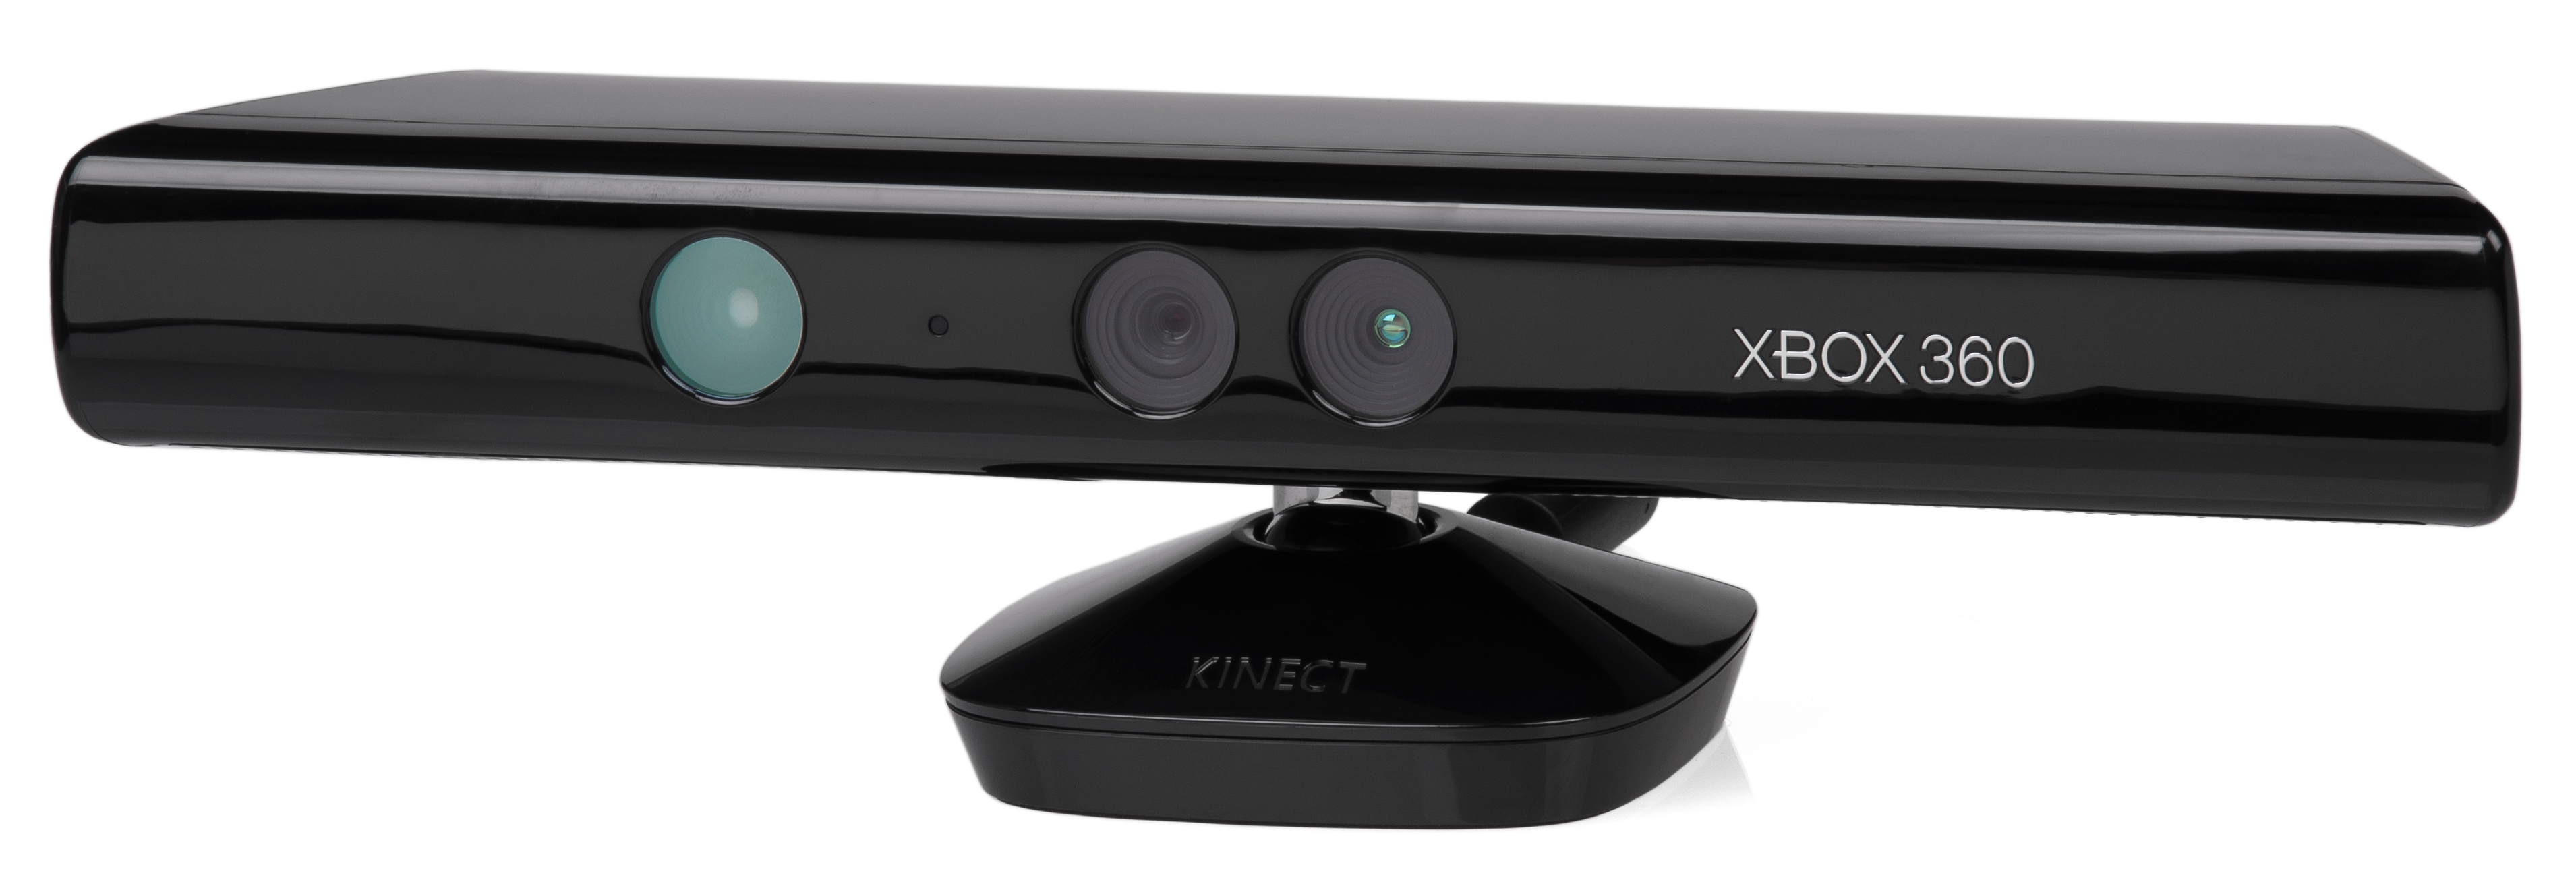
\includegraphics[width=0.4\linewidth]{imagens/kinect.png}
    \fonte{Disponível em: <https://pt.wikipedia.org/wiki/Kinect>. Acesso em 23 jun. 2025}
\end{figure}

Outra categoria relevante envolve controladores dedicados ao rastreamento manual, como o Leap Motion Controller (Figura \ref{leapmotion}). Zhang et al. (\citeyear{zhang2019gestureteleop}) demonstram sua aplicação em sistemas de teleoperação baseados em gestos, evidenciando a capacidade do dispositivo em detectar movimentos das mãos e dedos com alta precisão e baixa latência para aplicações em controle de robôs. Embora esse tipo de dispositivo ofereça alto desempenho para detecção de gestos precisos, ele também implica custo adicional de \textit{hardware} especializado, além de restringir o espaço de interação ao volume monitorado pelo sensor, o que contrasta com a meta do Aerochord de empregar soluções de baixo custo e maior flexibilidade.

\begin{figure}[htbp!]
	\caption{Controlador Leap Motion em uso para rastreamento de movimentos das mãos}
	\centering 
	\label{leapmotion}
	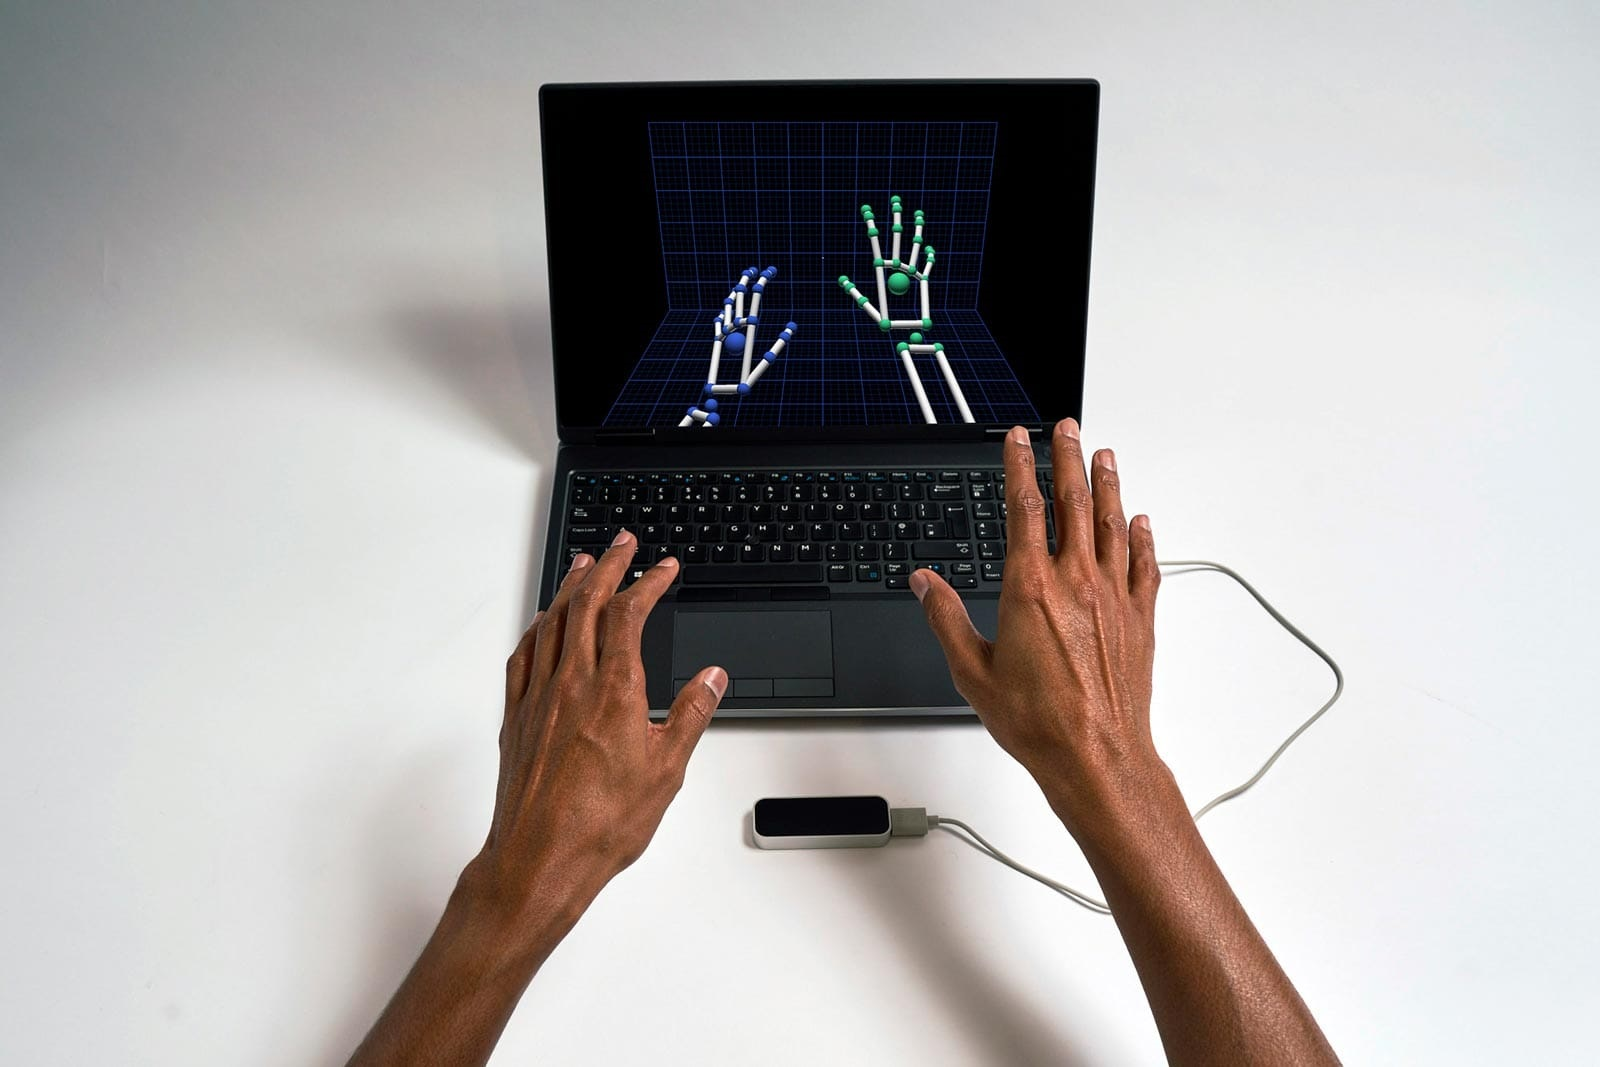
\includegraphics[width=0.55\linewidth]{imagens/LeapMotion.png}
    \fonte{Disponível em: <https://documentation.ls-group.fr/interact/LeapMotion/>. Acesso em 23 jun. 2025}
\end{figure}

No campo de sensores vestíveis (\textit{wearables}), destacam-se as chamadas luvas de dados (\textit{data gloves}) (Figura \ref{cyberglove}), que integram sensores de flexão e Unidades de Medição Inercial (IMUs) para medir diretamente os movimentos das mãos. A revisão feita por Dipietro et al. (\citeyear{dipietro2008survey}), aponta como pontos positivos a alta fidelidade na captura de ângulos articulares e ausência de problemas de oclusão visual, mas também ressalta desvantagens como o custo elevado, necessidade de calibração constante e caráter invasivo da interface, que pode prejudicar a naturalidade da interação. Essa categoria, embora tecnicamente robusta, também se afasta do objetivo do Aerochord de oferecer expressão musical sem impor acessórios ao usuário.

\begin{figure}[htbp!]
	\centering
	\caption{Luva de dados CyberGlove III projetada pela CyberGlove Systems}
	\label{cyberglove}
    \begin{subfigure}{0.36\textwidth}
		\centering
		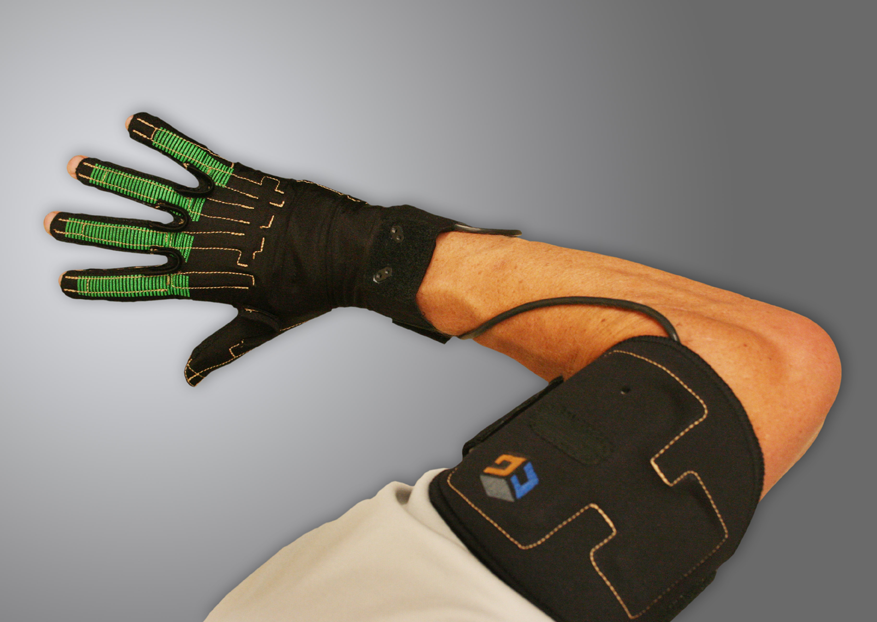
\includegraphics[width = \textwidth]{imagens/CyberGloveIII.png}
		\caption{Sensor vestível CyberGlove III}
		\label{fig:cyberglove_sensor}
	\end{subfigure}
    \begin{subfigure}{0.50\textwidth}
		\centering
		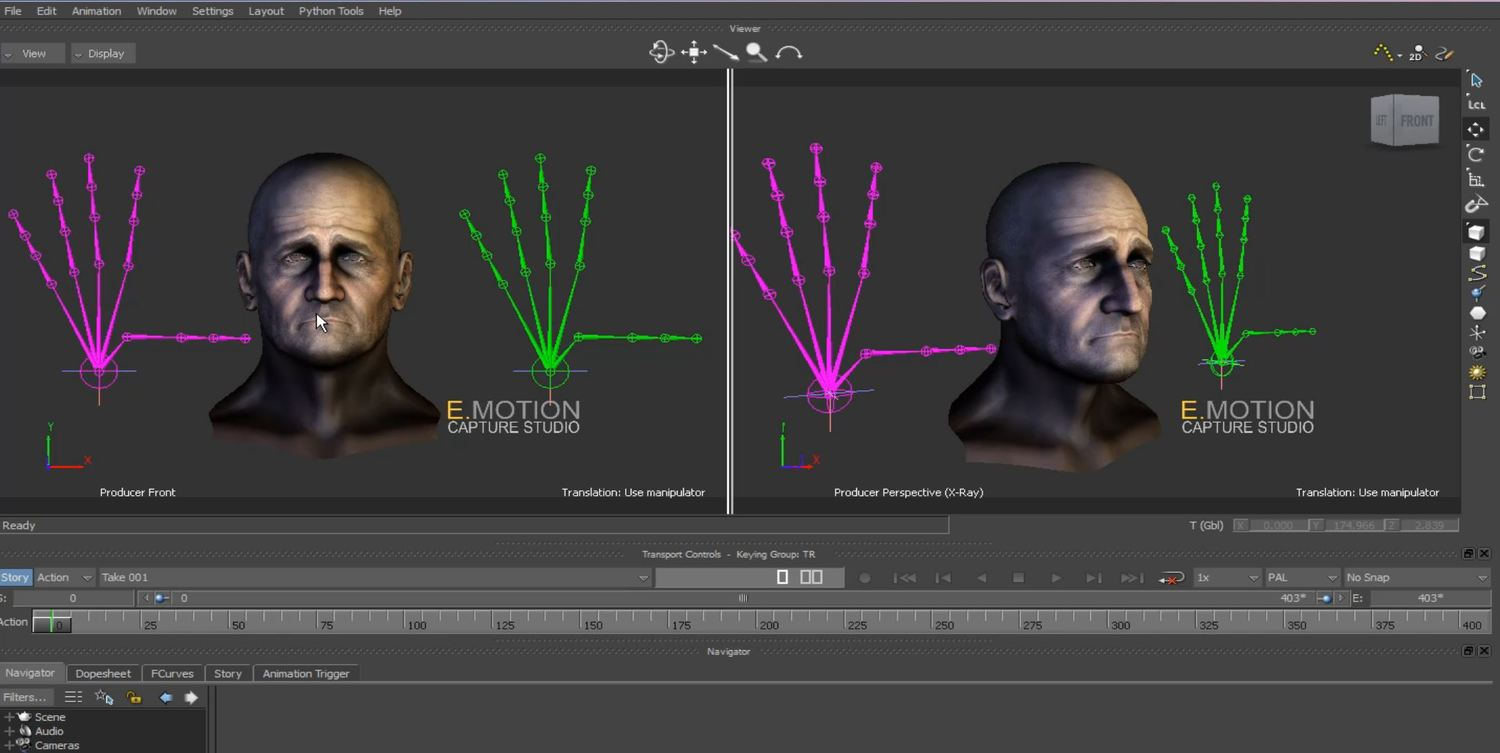
\includegraphics[width = \textwidth]{imagens/software_cyber_glove.jpg}
		\caption{\textit{Software} interpretando os comandos enviados pela CyberGlove III}
		\label{fig:cyberglove_software}
	\end{subfigure}
	\fonte{Disponível em: <https://www.cyberglovesystems.com/cyberglove-iii/>. Acesso em 23 jun. 2025}
\end{figure}

Adicionalmente, avanços em inteligência artificial e visão computacional têm viabilizado o rastreamento de gestos utilizando apenas câmeras RGB comuns, como \textit{webcams}. Rautaray e Agrawal (\citeyear{rautaray2012vision}) apresentam uma revisão de técnicas de reconhecimento de gestos baseadas em visão, destacando fases de detecção, rastreamento e reconhecimento que exploram desde segmentação de pele até modelos de aprendizado profundo (\textit{deep learning}) para extrair características das mãos em imagens bidimensionais (2D). Essa abordagem mostra-se promissora para aplicações acessíveis, uma vez que aproveita \textit{hardware} amplamente disponível e avanços em algoritmos que toleram variações de iluminação e cenários diversos, conectando-se diretamente ao objetivo do Aerochord de democratizar o controle gestual musical.

Entre as ferramentas de visão computacional para detecção de gestos, destaca-se o MediaPipe, \textit{framework} de código aberto (\textit{open source}) desenvolvido pelo Google, que oferece esteiras de processamento (\textit{pipelines}) pré-configuradas de aprendizado de máquina (\textit{machine learning}) para rastreamento de mãos e poses corporais em tempo real. Conforme descrito por Lugaresi et al. (\citeyear{lugaresi2019mediapipe}), o MediaPipe permite construir grafos de processamento de vídeo que interpretam o fluxo capturado pela \textit{webcam} e entregam, em tempo real, coordenadas tridimensionais (3D) estimadas dos pontos-chave das mãos, com desempenho otimizado para várias plataformas. A documentação oficial do projeto também fornece instruções detalhadas para a personalização e integração desses módulos em aplicações específicas \cite{mediapipeWebsite}. Por combinar alta precisão, baixa latência e depender apenas de \textit{hardware} onipresente, o MediaPipe consolidou-se como a base tecnológica do Aerochord, atendendo perfeitamente aos requisitos de expressividade musical e acessibilidade pretendidos.

\section{Hiperinstrumentos Musicais}
\label{sec:hiperinstrumentos_musicais}

A evolução dos instrumentos musicais na era digital pode ser entendida como uma extensão da longa história de refinamento das interfaces físicas entre o artista e o som, agora estendendo-se para além das restrições mecânicas e acústicas tradicionais em direção a sistemas computadorizados que ampliam as possibilidades expressivas. Conforme argumentado por Wanderley (\citeyear{wanderley2001gestural}), instrumentos digitais não sofrem as mesmas limitações físicas de tubos, cordas ou membranas, permitindo uma diversidade enorme de métodos de produção sonora. No entanto, para que esses sistemas ofereçam controle refinado comparável ao das famílias acústicas clássicas, estratégias de projeto cuidadosas de mapeamento e de interface devem ser definidas.

\subsection{Definição e Características}
\label{sec:definicao_e_caracteristicas}

Em 1986, Tod Machover fundou o grupo Hyperinstruments no \textit{MIT Media Lab}, formalizando o conceito de hiperinstrumento como uma extensão tecnológica da prática musical. Segundo o autor,  esse tipo de sistema é composto por três elementos fundamentais: (1) uma interface sensorial para o \textit{performer}\footnote{Pessoa que executa um instrumento, seja ele tradicional ou digital (\textit{performer}).}, capaz de capturar gestos, toques ou outras ações; (2) um módulo de processamento, que analisa e interpreta os dados de performance em tempo real; e (3) um sistema de geração ou modulação sonora, que pode envolver síntese digital, modelagem física ou controle de sintetizadores via protocolos como MIDI \cite{Machover1992}. No contexto do Aerochord, esses três componentes alinham-se da seguinte forma: a interface é o corpo do usuário capturado por visão computacional; o módulo de processamento é o \textit{software} em C++ que extrai pontos-chave e gestos (via MediaPipe); e o gerador sonoro pode ser qualquer sintetizador compatível com MIDI 2.0, acionado via \textit{Universal MIDI Packets}.

Machover (\citeyear{Machover1992}) enfatiza também a filosofia de aumentação em vez de mera substituição: não se trata apenas de criar timbres novos, mas de capturar nuances da performance humana (velocidade, aceleração, pressão, gestos sutis) que muitas vezes ficam fora do alcance de controles convencionais, e usar esses dados para controlar parâmetros sonoros de forma rica e multidimensional. Essa perspectiva de ampliar a expressividade natural do \textit{performer} reflete o objetivo de hiperinstrumentos de explorar dimensões de controle além do que um instrumento acústico isolado permitiria, usando o poder computacional para traduzir sutilezas gestuais em transformações sonoras complexas.

\subsection{Evolução e Exemplos Notáveis}
\label{sec:evolucao_e_exemplos_notaveis}

Historicamente, desvincular o gesto da produção sonora mecânica precede a era dos computadores. Instrumentos como o Theremin (Figura \ref{theremin}), criado em 1920, e o Ondes Martenot, desenvolvido em 1928, romperam com a necessidade de contato físico direto, permitindo o controle de altura e volume ou de timbre e efeito de modulação de frequência (\textit{vibrato}) por gestos. No caso do Theremin, a proximidade das mãos em relação às antenas determinava as frequências geradas, enquanto o Ondes Martenot combinava um teclado com um anel deslizante para manipulação contínua de som. Esses instrumentos pioneiros anteciparam, em termos conceituais, a performatividade expandida dos hiperinstrumentos computadorizados, ao sugerirem novas formas de mediação gestual e controle expressivo \cite{Manning1993}.

\begin{figure}[htbp!]
	\caption{Léon Theremin, criador do Theremin, demonstrando seu instrumento}
	\centering 
	\label{theremin}
	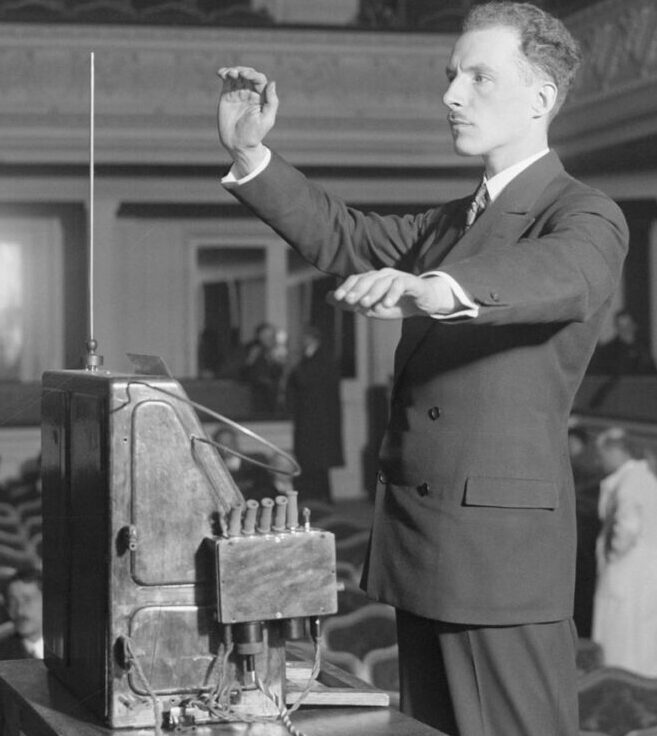
\includegraphics[width=0.24\linewidth]{imagens/theremin.jpg}
    \fonte{Disponível em: <https://en.wikipedia.org/wiki/Leon\_Theremin>. Acesso em 23 jun. 2025}
\end{figure}

A formalização do termo “hiperinstrumento” ocorreu em 1986, com o trabalho do grupo Hyperinstruments de Tod Machover. Um dos projetos mais emblemáticos desse período foi o Hypercello (Figura \ref{hypercello}), desenvolvido em 1991 por Machover em colaboração com o violoncelista Yo-Yo Ma, em que sensores no arco e no violoncelo capturavam parâmetros de performance (como pressão, velocidade e posição) e os convertiam em dados interpretados em tempo real para modificar aspectos do som, incluindo timbre, espacialização e efeitos. Esse modelo demonstra a aplicação prática dos três componentes definidos por Machover: o intérprete interage fisicamente (sensores no instrumento acústico), o computador processa os dados em tempo real, e o sistema sonoro responde de acordo com mapeamentos definidos, muitas vezes enriquecidos por algoritmos de síntese e processamento que ampliam o leque expressivo do instrumento original \cite{Machover1992}.

Em complemento aos projetos iniciais de Machover, Manning (\citeyear{Manning1993}) descreve também o \textit{Hyperbow Controller} (Figura \ref{hyperbow}), um arco de violino desenvolvido para uso com um violino elétrico. Esse dispositivo incorpora extensômetros (\textit{strain gauges}, sensores que medem deformação física) que medem as forças aplicadas no arco e acelerômetros que capturam variações de aceleração e inclinação durante o movimento. Essas informações gestuais são convertidas em múltiplos sinais de controle, que são processados em tempo real para modificar parâmetros como timbre, dinâmica e espacialização, sem comprometer a interação física familiar ao violinista. O \textit{Hyperbow} exemplifica a filosofia de aumentação em hiperinstrumentos, ampliando as possibilidades expressivas do gesto de arco tradicional ao traduzi-lo em comandos sonoros multidimensionais via síntese digital ou processamento computacional.

\begin{figure}[htbp!]
    \caption{Tod Machover e seu Hypercello}
    \centering 
    \label{hypercello}
    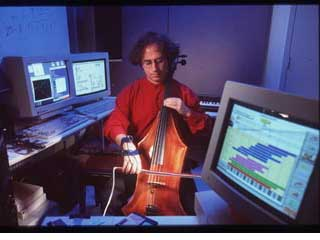
\includegraphics[width=0.75\linewidth]{imagens/hypercello.jpg}
    \fonte{Disponível em: <https://opera.media.mit.edu/projects/trilogy.html>. Acesso em 23 jun. 2025}
\end{figure}

\begin{figure}[htbp!]
    \caption{Hyperbow sendo utilizado em um violoncelo}
	\centering
    \label{hyperbow}
    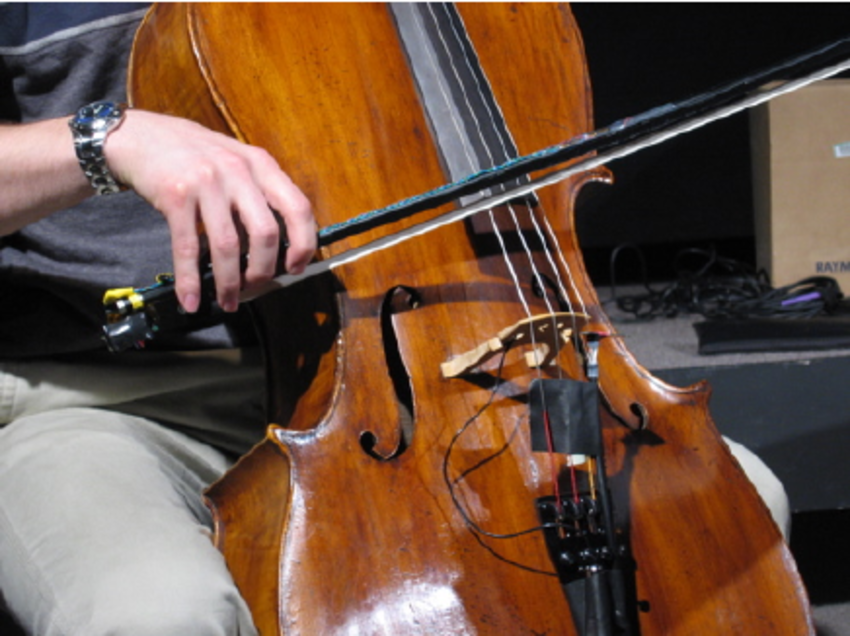
\includegraphics[width=0.6\linewidth]{imagens/hyperbow.png}
    \fonte{Disponível em: <https://www.researchgate.net/figure/Hyperbow-and-acoustic-acoustic-cello-C-Roberto-Aimi-Interestingly-although-the\_fig1\_221164872>. Acesso em 23 jun. 2025}
\end{figure}

Em tempos mais recentes, surgiram exemplos que empregam interfaces tangíveis e visuais para enriquecer a performance musical. Um exemplo é o Reactable (Figura \ref{reactable}), desenvolvido na \textit{Universitat Pompeu Fabra}, que consiste em uma superfície interativa sensível ao toque e à manipulação de objetos físicos, com visualização em tempo real para múltiplos usuários colaborarem musicalmente. Essa plataforma une o gesto manual direto a \textit{feedback} audiovisual, configurando uma forma contemporânea de hiperinstrumento que amplia a expressividade e a interação social em performance ao vivo \cite{weinerzl2017musical21}. Embora existam também controladores gestuais baseados em \textit{hardware} dedicado, a ênfase recente em visão computacional e sensores amplamente disponíveis reflete a busca por acessibilidade, alinhando-se diretamente ao projeto Aerochord, que visa empregar câmeras comuns para capturar gestos e oferecer controle musical sensível sem exigir dispositivos especializados.

\begin{figure}[htbp!]
    \caption{Reactable}
	\centering
    \label{reactable}
    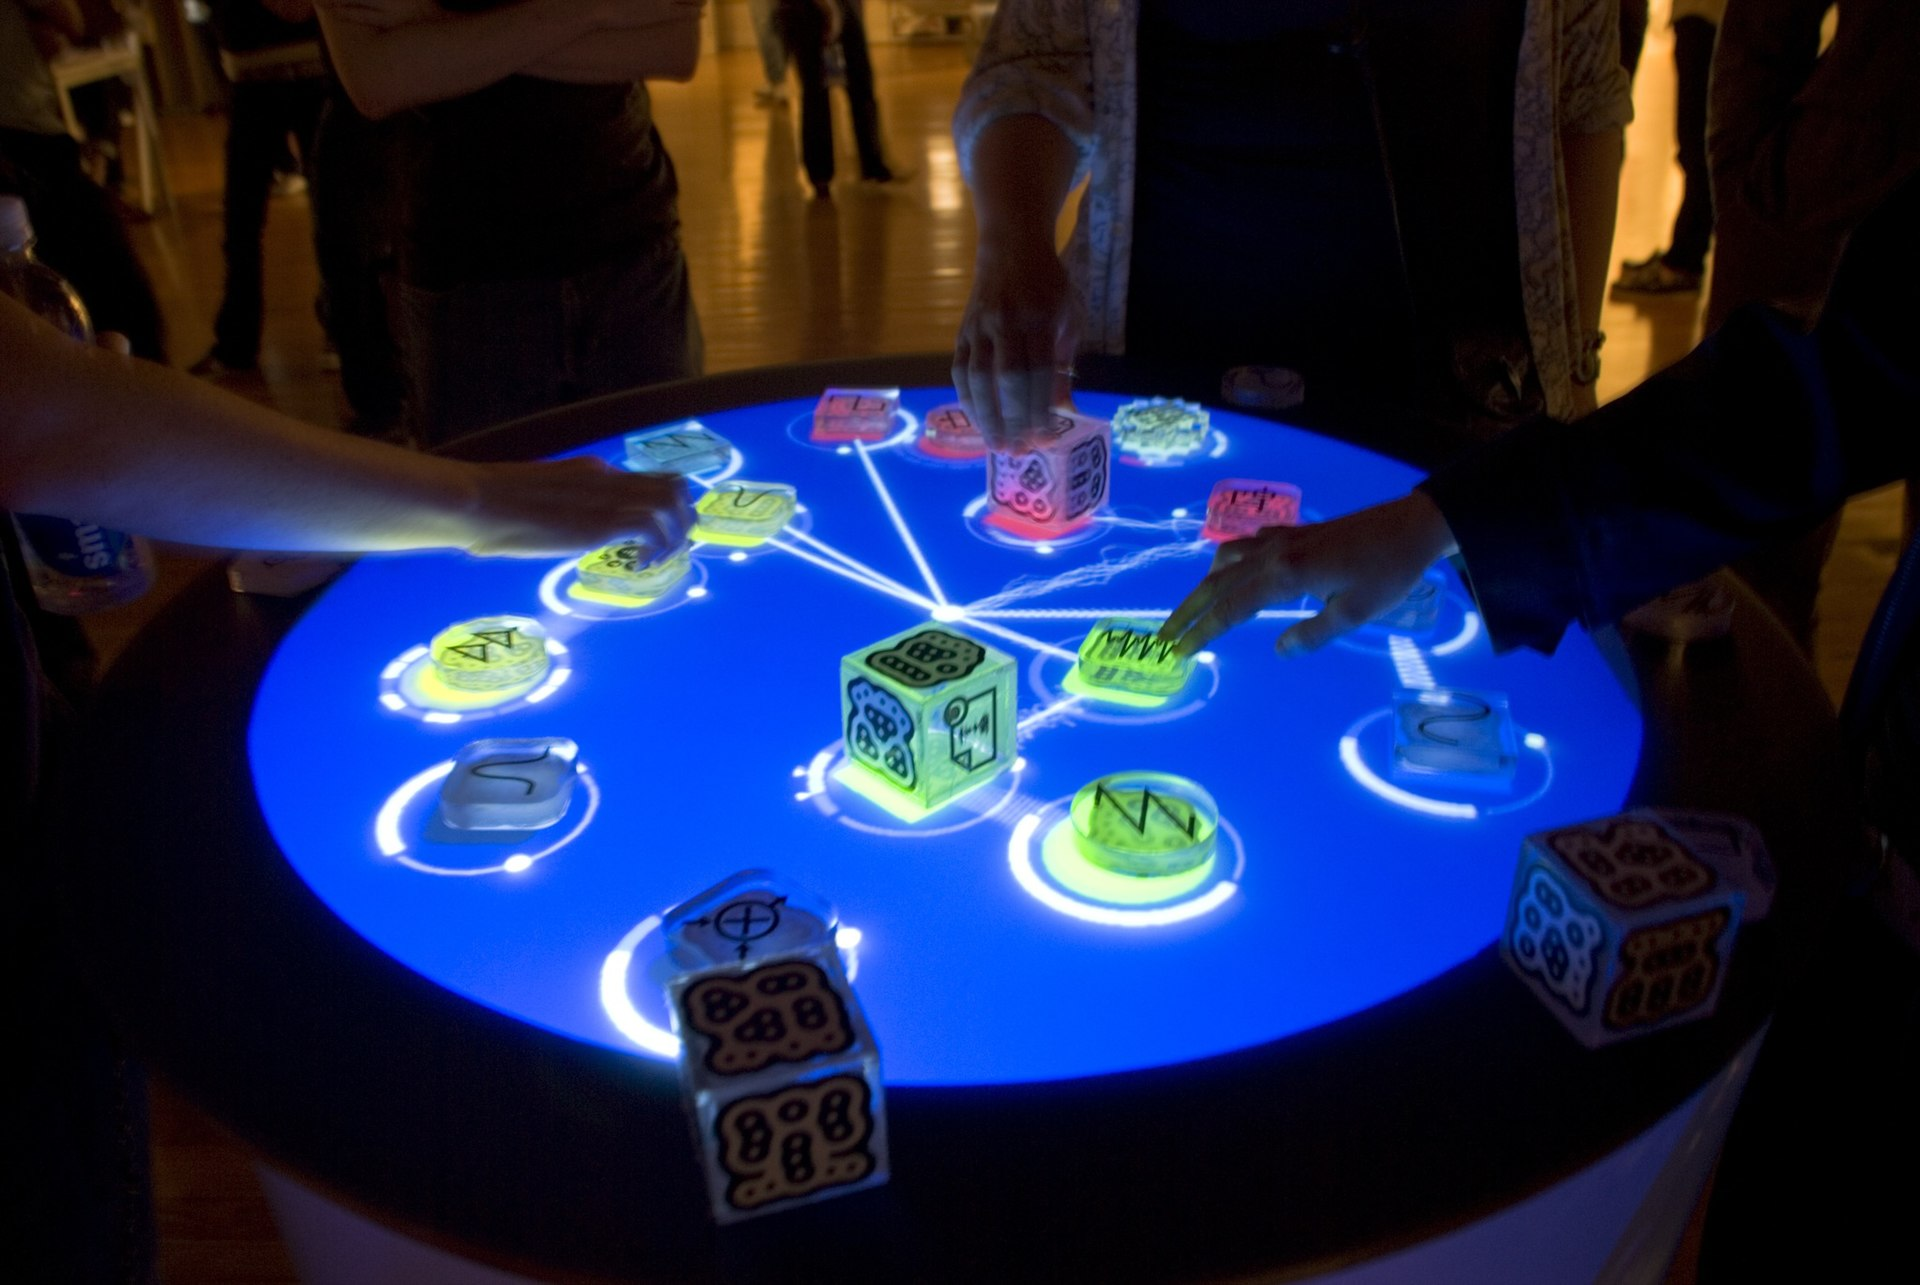
\includegraphics[width=0.5\linewidth]{imagens/reactable.jpg}
    \fonte{Disponível em: <https://en.wikipedia.org/wiki/Reactable>. Acesso em 23 jun. 2025}
\end{figure}

\subsection{Hiperinstrumentos e Interação Gestual}
\label{sec:hiperinstrumentos_e_interacao_gestual}

A interação gestual ocupa papel central no \textit{design} de hiperinstrumentos, pois permite capturar a expressividade natural do corpo do \textit{performer} de modo contínuo e multidimensional. Conforme argumenta Wanderley (\citeyear{wanderley2001gestural}), o gesto musical, especialmente em instrumentos acústicos, já é uma forma de controle multiparamétrico, envolvendo aspectos como sincronização rítmica (\textit{timing}), articulação e dinâmica. Transportar essa riqueza para interfaces digitais exige que o sistema capture variações sutis de velocidade, aceleração e posição, assegurando um mapeamento claro e responsivo entre gesto e som. 

No Aerochord, a adoção da visão computacional com MediaPipe exemplificou perfeitamente essa proposta. Ao extrair coordenadas 3D das mãos em tempo real, o sistema preserva a latência e a precisão necessárias para a expressividade musical. Entretanto, o verdadeiro desafio superado esteve no \emph{mapeamento}: isto é, na definição de regras que traduzem os dados gestuais em parâmetros sonoros de forma musicalmente coerente e criativa. Wanderley (\citeyear{wanderley2001gestural}) destaca que um mapeamento eficaz deve respeitar propriedades perceptivas e ergonômicas, oferecer consistência e previsibilidade (para aprendizado do \textit{performer}), mas também permitir explorabilidade para descobertas sonoras. No contexto de hiperinstrumentos, o mapeamento implementado no projeto não foi apenas linear, envolvendo fusão de múltiplas dimensões gestuais que dialogam diretamente com as extensões proporcionadas pelo MIDI 2.0.

\section{Considerações sobre o Capítulo}
\label{sec:consideracoes_sobre_o_capitulo}

Ao longo deste capítulo, fundamentou-se o projeto Aerochord em pilares teóricos que se articulam de modo coeso: inicialmente, a partir dos princípios da IHC que enfatizam a busca por interfaces mais naturais e centradas no usuário; em seguida, pela caracterização da interação gestual como uma modalidade de controle especialmente poderosa e expressiva; e, finalmente, pela concepção dos hiperinstrumentos como modelo ideal para explorar essa expressividade no domínio musical. Essa jornada conceitual reforça que o Aerochord não é uma iniciativa isolada, mas sim o resultado de uma proposta fundamentada em princípios consolidados da computação musical e da IHC.

A relevância contemporânea desse enquadramento revela-se na convergência entre a ambição histórica dos hiperinstrumentos de Machover, originalmente dependentes de sensores dedicados, \textit{hardware} especializado e ambientes de pesquisa de alto custo, e o advento de ferramentas de visão computacional de código aberto (\textit{open source}), como o MediaPipe, que operam com \textit{hardware} genérico (por exemplo, uma simples \textit{webcam}). Enquanto Machover (\citeyear{Machover1992}) descreveu hiperinstrumentos cuja expressividade exigia infraestrutura complexa, o panorama atual oferece camadas de percepção corporal em tempo real, robustas e acessíveis \cite{lugaresi2019mediapipe}. Foi precisamente nessa interseção (entre o conceito expressivo de hiperinstrumento e a democratização tecnológica) que o Aerochord se estabeleceu, viabilizando a mesma amplitude de controle de projetos pioneiros de maneira acessível a criadores sem necessidade de equipamentos exclusivos.

Os hiperinstrumentos representam a convergência de pesquisas em interação gestual, processamento de sinais e \textit{design} de interface musical, cujo objetivo é ampliar as capacidades expressivas do \textit{performer}. Desde pioneiros como Theremin e Ondes Martenot até plataformas modernas baseadas em visão computacional e interfaces tangíveis (como o Reactable), observa-se um fio condutor claro: a busca por interfaces que respondam ao corpo do artista com sensibilidade e precisão enquanto oferecem liberdade criativa ampliada pelo poder computacional. As escolhas de tecnologia realizadas no Aerochord foram integralmente orientadas pelos princípios da expressividade musical e da usabilidade performática.

Entretanto, mesmo com o suporte teórico consolidado e a disponibilidade de tecnologia acessível, o sucesso de qualquer hiperinstrumento gestual repousa no desafio central do mapeamento gestual, isto é, da tradução entre movimento corporal e transformação sonora. Como enfatizado em Wanderley \citeyear{wanderley2001gestural}, o mapeamento constitui o ``coração'' de um instrumento digital gestual: ele deve ser suficientemente intuitivo para iniciantes e profundo o bastante para permitir aos músicos experientes explorar dimensões expressivas mais sutis (velocidade, aceleração, forma de movimento, variações dinâmicas). 

O Capítulo~\ref{chap:desenvolvimento_proposta} detalha como o Aerochord abordou e superou esse desafio na prática, descrevendo a arquitetura de \textit{software} implementada e as estratégias projetadas para equilibrar usabilidade e riqueza expressiva.
\chapter{Computação e Música}
\label{cap:computacao_musical}

Este capítulo apresenta a base teórica que serviu de apoio para o desenvolvimento da solução computacional do Aerochord. Na Seção~\ref{sec:fundamentos_computacao_musical}, discutem-se os fundamentos da computação musical, incluindo representação digital do som, síntese sonora e processamento de áudio digital. Em seguida, a Seção~\ref{sec:protocolo_midi} detalha o protocolo MIDI (Interface Digital para Instrumentos Musicais, do inglês \textit{Musical Instrument Digital Interface}), apresentando seu propósito, funcionamento e as mensagens mais relevantes para o controle expressivo do sistema. Por fim, na Seção~\ref{sec:teoria_musical}, revisam-se os principais conceitos de teoria musical aplicados ao mapeamento gestual — escala cromática, oitavas, articulações (notas curtas e destacadas, \textit{staccato}; ou notas fluidas e ligadas, \textit{legato}) e efeitos como modulação de afinação e frequência (\textit{pitch bend} e \textit{vibrato}), sustentação (\textit{sustain}) e dinâmica — que fundamentaram o \textit{design} do instrumento.

\section{Fundamentos da Computação Musical}
\label{sec:fundamentos_computacao_musical}

A computação musical concentra-se na aplicação de algoritmos e modelos computacionais para criar, analisar e modificar sons de maneira flexível e precisa. Conforme destacado por Miranda (\citeyear{Miranda2002}), esse campo abrange desde a geração programada de timbres até a modelagem de estruturas musicais complexas e sistemas de execução (\textit{performance}) interativa. Dodge e Jerse (\citeyear{Dodge1997}) enfatizam o papel do computador na realização de tarefas sonoras avançadas, enquanto Moore (\citeyear{Moore1990}) evidencia a importância da representação digital do som, permitindo seu armazenamento e processamento eficientes.

O processo inicia-se com a conversão de um sinal analógico em dados numéricos, por meio de dois estágios principais: a amostragem, que mede a amplitude do sinal em instantes regulares, e a quantização, que mapeia essas medições para valores discretos \cite{Rossing2002}. Essa sequência de valores numéricos serve de base para todas as operações subsequentes.

A síntese sonora gera sons por meio de modelos computacionais em vez de gravações acústicas. Na síntese aditiva, ondas senoidais puras são somadas para formar timbres; na síntese subtrativa, sinais ricos em harmônicos são filtrados para moldar o espectro sonoro. A modulação de frequência (FM) altera dinamicamente a frequência de uma portadora por uma moduladora, produzindo timbres expressivos, enquanto a síntese granular emprega pequenos fragmentos de áudio (os ``grãos'') para criar texturas sonoras singulares \cite{Manning1993}.

O processamento de áudio digital manipula gravações pré-existentes por meio de técnicas como filtragem, equalização, compressão, reverberação e aplicação de efeitos especiais, aprimorando a qualidade sonora e possibilitando transformações criativas \cite{Zolzer2011}. Essas operações são largamente empregadas em Estações de Trabalho de Áudio Digital (\textit{Digital Audio Workstations} - DAWs) para modelar o som conforme a intenção artística.

As aplicações da computação musical incluem a criação de instrumentos digitais equipados com sensores e controladores, a composição assistida por computador que apoia o desenvolvimento de ideias melódicas e estruturais, e sistemas interativos que respondem em tempo real aos gestos do intérprete (\textit{performer}). Adicionalmente, métodos de análise e recuperação de informação musical permitem indexar e buscar repertórios com base em atributos como melodia, ritmo e timbre \cite{Cope2001}.

No contexto deste trabalho, esses fundamentos habilitaram a captação e interpretação de gestos corporais e seu mapeamento para mensagens MIDI coerentes. A etapa de quantização assegurou precisão na conversão dos sinais de movimento, enquanto a síntese e o processamento digital compõem o ambiente sonoro no \textit{software} receptor. Ao integrar esses elementos, o hiperinstrumento desenvolvido amplia as possibilidades expressivas do intérprete, tornando seu corpo parte ativa da criação musical.

\section{O Protocolo MIDI (Musical Instrument Digital Interface)}
\label{sec:protocolo_midi}

Desde seu surgimento em meados de 1983, o protocolo MIDI estabeleceu-se como padrão onipresente para comunicação de eventos musicais entre controladores, sintetizadores e sequenciadores, permitindo que equipamentos de fabricantes distintos interagissem de forma consistente e interoperável \cite{SMC2023MIDI,MIDI1DetailedSpec}. Essa universalidade viabilizou a criação de um ecossistema diversificado de equipamentos físicos (\textit{hardware}) e lógicos (\textit{software}), moldando práticas de produção, \textit{performance} e composição musical ao longo de décadas. Porém, à medida que as demandas por expressividade mais refinada, controle de alta precisão e interação em tempo real evoluíram, especialmente em contextos de performance gestual, tornaram-se evidentes limitações do MIDI 1.0, tais como resolução restrita de parâmetros, comunicação predominantemente unidirecional e ausência de mecanismos de autoconfiguração \cite{MIDI2Overview2023}.

Em cenários de interfaces musicais gestuais de baixa latência e alta expressividade, como o projeto Aerochord, essas restrições tornam-se especialmente críticas: o mapeamento fino de gestos a parâmetros sonoros exige curvas de resposta suaves, confirmação de capacidades do dispositivo receptor e sincronização precisa de eventos. Foi essa necessidade que motivou a adoção do MIDI 2.0 no projeto, cuja arquitetura revisada introduz inovações concebidas para atender a tais exigências sem abandonar a compatibilidade retroativa com o ecossistema existente. Nesta seção, são apresentados inicialmente os fundamentos e as limitações do protocolo MIDI 1.0. Em seguida, discute-se a arquitetura técnica e as novas capacidades do MIDI 2.0, demonstrando como elas fundamentaram a escolha desse protocolo como pilar tecnológico do Aerochord.

\subsection{Fundamentos e Limitações do MIDI 1.0}
O protocolo MIDI 1.0 opera como um sistema de transmissão de instruções musicais, transportando mensagens que indicam eventos sem veicular o áudio propriamente dito \cite{SMC2023MIDI,MIDI1DetailedSpec}. Os eventos mais comuns incluem ativação e desativação de notas (\textit{Note On} e \textit{Note Off}), intensidade do toque (\textit{Velocity}), mudanças de parâmetros de som (\textit{Control Change}), troca de instrumentos (\textit{Program Change}), dobra de afinação (\textit{Pitch Bend}) e mensagens exclusivas de fabricantes (\textit{System Exclusive} ou \textit{SysEx}). Cada mensagem é composta por um byte de estado (com bit alto indicando tipo de mensagem e canal) seguido de um ou dois bytes de dados (com 7 bits significativos), refletindo a concepção original de comunicação serial a 31,25 kbps. Essa taxa de transferência definia limites para o número de eventos simultâneos que poderiam ser enviados sem comprometer significativamente a latência ou gerar congestionamento na linha.

Ao unificar equipamentos de fabricantes distintos, o MIDI 1.0 estabeleceu um ecossistema interoperável, permitindo que controladores e DAWs compartilhassem mensagens comuns. Essa compatibilidade retroativa sustenta uma vasta base instalada de dispositivos e aplicou-se também ao Aerochord, que implementou a capacidade de enviar mensagens em modo legado a sintetizadores sem suporte a MIDI 2.0, assegurando que usuários com equipamentos existentes possam integrar o sistema sem barreiras.

Entretanto, para aplicações que demandam expressividade refinada e baixa latência a concepção original do MIDI 1.0 revela limitações críticas. A resolução de 7 bits em \textit{Control Changes} e \textit{Velocity} implica apenas 128 passos discretos, frequentemente resultando em saltos audíveis em variações contínuas; o \textit{Pitch Bend} afeta todas as notas de um mesmo canal simultaneamente, impedindo modulações individuais em acordes polifônicos; a comunicação é primordialmente unidirecional; o número restrito de 16 canais por porta limita distinções granulares; e a ausência de marcas de tempo (\textit{timestamps}) embutidas impede compensações automáticas de variações no tempo de chegada dos dados (\textit{jitter})\footnote{Variação no atraso da transmissão de dados sobre uma rede ou barramento, causando irregularidades e possíveis problemas de sincronização.}. Esses fatores se tornam especialmente significativos no Aerochord, em que a fluidez do mapeamento de gestos exigiu curvas suaves e sincronização precisa que ultrapassam o escopo do padrão legado \cite{MIDI2Overview2023}.

\subsection{Arquitetura Técnica do MIDI 2.0}
O surgimento do MIDI 2.0 representa uma resposta direta às limitações identificadas no protocolo legado, oferecendo compatibilidade retroativa ao introduzir mecanismos bidirecionais que permitem autoconfiguração e descoberta de capacidades entre instrumentos \cite{MIDI2Overview2023}. Essa evolução foi motivada pela necessidade de suportar demandas de expressividade refinada em tempo real, onde a fluidez gestual é um requisito central.

No cerne da nova arquitetura estão os Pacotes MIDI Universais (\textit{Universal MIDI Packets} - UMP), que redefinem o formato de mensagens para 32, 64 ou 128 bits, com campos que incluem tipo de mensagem, grupo, canal/comando e, opcionalmente, \textit{timestamp} embutido \cite{UMPProtocol2023}. Essa estrutura ampliada possibilita transportar dados de alta resolução e atuar com controladores por nota individual (\textit{per-note controllers})\footnote{Controladores que permitem ajustar parâmetros como volume, afinação e timbre de cada nota individualmente, diferentemente dos controles comuns que afetam todo o canal.}. No Aerochord, cada evento gestual é marcado com um \textit{timestamp} no momento exato da captura, propagado internamente por todo o \textit{pipeline} até o envio do pacote MIDI. Esse \textit{timestamp} é usado para medir a latência \textit{end-to-end} do sistema (percentis P50/P95) — ele não é serializado como mensagem de \textit{Jitter-Reduction Timestamp} dentro do próprio pacote UMP transmitido ao dispositivo receptor, ficando restrito à instrumentação interna do Aerochord.

A descoberta de capacidades passa a ser realizada por meio da Consulta de Capacidades MIDI (\textit{MIDI Capability Inquiry} - MIDI-CI), em que um dispositivo envia mensagens de busca e recebe detalhes sobre o suporte a MIDI 2.0 e propriedades configuráveis \cite{MIDICI2023}. Esse protocolo de negociação inicial (\textit{handshake}) transforma a comunicação "cega" em uma negociação inteligente: o Aerochord identifica automaticamente se o receptor aceita mensagens UMP, dispensando configurações manuais extensas.

Em sequência, os Perfis (\textit{Profiles}) e a Troca de Propriedades (\textit{Property Exchange}) permitem compartilhar conjuntos padronizados de regras. Os perfis definem como interpretar mensagens em contextos específicos (ex: mapeamentos para \textit{per-note controllers}), enquanto o \textit{Property Exchange} possibilita consultar e ajustar dinamicamente parâmetros remotos, como curvas de resposta, sem sair da sessão \cite{MIDICIProfiles2023,MIDIPropertyExchange2023}. 

A arquitetura também prevê flexibilidade de transporte: pacotes UMP podem trafegar via USB, \textit{Bluetooth} ou rede, ao mesmo tempo em que existe uma contingência (\textit{fallback}) para encapsular mensagens em conexões MIDI 1.0 legadas \cite{UMPProtocol2023}. Essa adaptabilidade garante operação em múltiplas plataformas, mantendo a funcionalidade básica mesmo em dispositivos antigos.

Por fim, a especificação prevê até 16 grupos independentes, cada um com 16 canais, permitindo separar fluxos de controle distintos. Como o Aerochord, em sua versão atual, é um instrumento monofônico de voz única — em que notas, volume, sustentação, timbre, vibrato e \textit{pitch bend} moldam o mesmo som —, todos os eventos das duas mãos são roteados para um único grupo e canal. Essa escolha garante que os macrocontroles globais (volume e sustentação, operados pela mão de controle) e as modulações por nota (operadas pela mão de articulação) incidam efetivamente sobre as notas em execução, uma vez que, na especificação, cada grupo constitui uma porta lógica de 16 canais independente. Os grupos adicionais permanecem reservados para a evolução polifônica e multivoz do sistema, discutida entre os trabalhos futuros (Capítulo~\ref{chap:consideracoes_finais}).

\subsection{Novas Capacidades Expressivas do MIDI 2.0}
Ao redefinir o formato e introduzir mecanismos de maior resolução, o MIDI 2.0 abre espaço para ganhos expressivos inimagináveis no padrão legado, os quais se refletiram diretamente no Aerochord \cite{MIDI2Overview2023,UMPProtocol2023}.

A alta resolução representa um avanço fundamental: valores de \textit{Velocity} passam a ter 16 bits e \textit{Control Changes} podem alcançar 32 bits, eliminando saltos audíveis. No Aerochord, onde pequenas alterações de gesto modulam contínua e simultaneamente vários efeitos, essa granularidade estendida assegurou que o mapeamento refletisse nuances sutis sem artefatos \cite{UMPProtocol2023}.

Outra capacidade expressiva é o suporte a controle por nota individual. Diferentemente do MIDI 1.0, o MIDI 2.0 permite enviar mensagens de afinação, modulação ou pressão após o toque (\textit{aftertouch}) para notas específicas dentro de um acorde. Esse recurso viabilizou que o Aerochord aplicasse afinação apenas a uma nota sustentada (\textit{UMP MT4 Opcode 0x6}), enquanto as outras permanecem estáveis, enriquecendo texturas polifônicas de modo antes inviável.

O transporte de blocos estruturados de dados torna-se mais robusto, permitindo enviar configurações e predefinições completas (\textit{presets}) de sintetizadores em formato padronizado. A padronização desses mecanismos facilita a portabilidade e a experimentação colaborativa, integrando-se à calibração dinâmica em tempo real \cite{MIDIPropertyExchange2023}. 

\subsection{Persistência de Performances e Arquivos}
Registrar performances gestuais com fidelidade é fundamental para edição e análise detalhada. Em instrumentos como o Aerochord, cada gesto traduzido em MIDI 2.0 contém dados de alta resolução e \textit{timestamps} que documentam a evolução temporal exata dos controles.

O formato Arquivo de Clipe MIDI (\textit{MIDI Clip File}), baseado em UMP, oferece suporte à gravação de sequências contendo mensagens de alta resolução e \textit{timestamps} embutidos \cite{MIDIClipFile2023}. Em complemento, o Arquivo Contêiner (\textit{Container File}) permite agrupar múltiplos clipes e metadados, formando um pacote coeso. 

No contexto de avaliação do Aerochord, a persistência de eventos (implementada através do modo de avaliação analítica, \textit{eval mode}, exportando para arquivos tabulares) e os registros (\textit{logs}) precisos de eventos de ponta a ponta (\textit{end-to-end}) desempenharam um papel vital na medição de latência e de precisão do sistema.

\subsection{Justificativa Final para a Arquitetura do Aerochord}
Em síntese, as capacidades do MIDI 2.0 — alta resolução, controle por nota individual, autoconfiguração via MIDI-CI e \textit{timestamps} — atenderam diretamente aos requisitos de expressividade e robustez que nortearam o Aerochord \cite{UMPProtocol2023,MIDICI2023,MIDIPropertyExchange2023,MIDIClipFile2023}.

Em termos de aplicação concreta, a distância entre os dedos pôde controlar filtros sonoros suavemente sem saltos audíveis. Ao sustentar acordes, gestos de vibração geraram modulação independente em notas específicas. Além disso, ao conectar-se internamente, o Aerochord integrou uma porta virtual em modo MIDI 2.0, configurando parâmetros (\textit{setup}) de forma transparente.

O suporte a MIDI 2.0 não foi meramente um recurso opcional, mas o elemento central para viabilizar o controle gestual de alta precisão alcançado. A adoção do padrão potencializou a missão de democratização, oferecendo uma exploração fina com resposta sonora refinada.

\section{Teoria Musical Aplicada}
\label{sec:teoria_musical}

Esta seção apresenta os fundamentos da teoria musical que serviram de base para o mapeamento gestual no sistema Aerochord. Serão abordados os conceitos de escala cromática e oitavas \cite{benward2014music}. Em seguida, noções de articulação, como \textit{staccato} e \textit{legato} \cite{duckworth2015creative}. Por fim, revisam-se efeitos como \textit{vibrato, pitch bend, sustain} e dinâmica, implementados a partir das variações nos gestos captados \cite{Dodge1997}.

\subsection{Escala Cromática e Oitavas}
\label{sec:teoria_musical_escalas}

A escala cromática consiste na divisão da oitava em doze semitons iguais, representando a menor unidade de distância entre duas notas no sistema temperado. Cada semitom equivale a um aumento fixo de frequência, criando um sistema padronizado \cite{benward2014music}.

No contexto do MIDI, cada nota é representada por um número inteiro de 0 a 127. A nota Dó central (C4 ou MIDI 60) serve como referência, onde aumentos de valor representam semitons sucessivos. As oitavas são formadas por doze semitons (relação de frequência 2:1), percebidas como uma repetição da mesma nota em um registro mais agudo \cite{duckworth2015creative}. Essa percepção invariável foi explorada no Aerochord por meio dos gestos de seleção.

Do ponto de vista do \textit{design} gestual, o mapeamento suporta usuários destros e canhotos sem qualquer configuração prévia: os papéis de cada mão (controle vs.\ articulação) são atribuídos pela ordem de entrada em quadro, e não pela lateralidade anatômica do usuário (ver Seção~\ref{sec:captura_deteccao}). A altura vertical do quadro de visão da câmera foi dividida em doze zonas discretas (semitons) ativadas pela \textbf{mão de articulação} (a segunda mão a entrar em quadro). Simultaneamente, movimentos verticais macro da \textbf{mão de controle} (a primeira a entrar) determinavam a transição entre oitavas. Isso possibilitou ao usuário navegar por registros diferentes de forma ergonômica, escolhendo livremente qual mão usar para cada papel.

\subsection{Articulações}
\label{sec:teoria_musical_articulacoes}

As articulações musicais determinam como as notas se conectam. O \textit{staccato} indica notas breves e destacadas. No Aerochord, esse efeito é reproduzido por movimentos rápidos e secos, como um fechamento súbito dos dedos seguido de uma liberação imediata, gerando notas curtas \cite{duckworth2015creative}.

Por outro lado, o \textit{legato} indica uma execução fluida. Em termos técnicos, significa a emissão de um \textit{Note On} antes do \textit{Note Off} da nota anterior, criando sobreposição. No Aerochord, isso foi interpretado permitindo o deslize da mão de articulação fechada entre as zonas verticais de nota. Essa abordagem exigiu lógica computacional precisa para gerir as fronteiras, utilizando zonas mortas (\textit{dead zones} - áreas de tolerância de entrada) e configurações de estabilização do sinal para evitar ativações duplas indesejadas \cite{benward2014music}.

\subsection{Efeitos de expressividade}
\label{sec:teoria_musical_efeitos}

A expressividade musical reflete a resposta a nuances da execução. O \textit{vibrato} é a modulação periódica na frequência da nota. No MIDI 2.0, seu controle opera com alta granularidade \cite{midi_org}. No Aerochord, esse efeito foi gerado a partir de pequenos movimentos oscilatórios laterais da mão de articulação durante a ativação da nota.

O \textit{pitch bend} altera a afinação de forma contínua. Tratado como \textit{Per-Note Pitch Bend} (atributo por nota) em MIDI 2.0, o sistema interpretou deslocamentos angulares de inclinação da mão de articulação para realizar transições melódicas fluídas, mapeando a rotação diretamente para o valor de afinação da nota em andamento \cite{midi_org}.

O \textit{sustain} refere-se à capacidade de manter o som após o término da ação física. A manutenção da \textbf{mão de controle} aberta (em repouso vertical temporário) foi mapeada para acionar e desativar o \textit{sustain}, garantindo que as notas ativadas pela \textbf{mão de articulação} pudessem permanecer soando de maneira análoga ao pedal de sustentação de um piano.

A dinâmica diz respeito à intensidade sonora (comumente tratada na música tradicional sob termos como \textit{piano}, \textit{forte} e \textit{crescendo}). No protocolo MIDI, a dinâmica do ataque da nota é controlada pelo \textit{velocity}. No projeto, a velocidade de fechamento dos dedos da mão de articulação (distância mensurada em janelas de tempo) foi calculada pelo \textit{software} e mapeada para a intensidade da nota, permitindo ataques percussivos suaves ou agressivos conforme a intenção do usuário \cite{benward2014music}.

\section{Considerações sobre o Capítulo}
\label{sec:consideracoes_cap3}

Ao longo deste capítulo, foram apresentados os fundamentos da computação musical e explorado o protocolo MIDI. Demonstrou-se como o MIDI 2.0 reverteu obstáculos de baixa resolução por meio de pacotes universais (UMP) e consultas automáticas (MIDI-CI).

A compreensão dessas especificações técnicas constituiu o alicerce sobre o qual a arquitetura de \textit{software} do Aerochord se apoiou. A capacidade de endereçar dados de alta resolução e controlar a afinação (\textit{pitch bend}) de cada nota individualmente foi o elemento-chave que viabilizou o mapeamento fluido implementado.

Com os conceitos de IHC, teoria musical e protocolo MIDI firmemente estabelecidos, o Capítulo~\ref{cap:analise_estado_arte_interfaces_musicais_gestuais} aprofundará a revisão da literatura, examinando soluções existentes para delimitar exatamente o cenário onde a proposta de solução (detalhada no Capítulo~\ref{chap:desenvolvimento_proposta}) foi implementada.
\chapter{Estado da Arte em Interfaces Musicais Gestuais}
\label{cap:analise_estado_arte_interfaces_musicais_gestuais}

Uma análise do estado da arte em interfaces musicais gestuais deve ir além da simples catalogação de tecnologias e dispositivos: é preciso centrar a investigação nos paradigmas de interação que essas soluções viabilizam e nas concessões mútuas (\textit{trade-offs}) implícitas em cada abordagem. Essa perspectiva não se limita a enumerar sensores, bibliotecas ou arcabouços de desenvolvimento (\textit{frameworks}), mas busca compreender como, historicamente e atualmente, diferentes formas de captação gestual, mapeamento e entrega de retorno sensorial (\textit{feedback}) procuram equilibrar três pilares cruciais: a fidelidade na captura dos gestos, a expressividade resultante no domínio sonoro e a acessibilidade de uso para perfis diversos de usuários.

Este capítulo segue uma narrativa estruturada em etapas complementares. Primeiramente, é explorado como paradigmas clássicos — de sistemas baseados em contato físico dedicado a gestos livres em espaço tridimensional ou a capturas por visão monocular — moldaram o que hoje se entende como possibilidades e limitações em interfaces musicais gestuais. Em seguida, discute-se o desafio central do mapeamento gesto–som, investigando tanto estratégias discretas e contínuas, bem como filosofias de projeto (\textit{design}) orientadas a priorizar o movimento (\textit{movement-first}) ou priorizar o som (\textit{sound-first}). Na sequência, exploram-se métodos de avaliação, perfis de usuário e cenários de aplicação, situando cada abordagem em contextos reais e em requisitos de usabilidade, latência e expressividade. Por fim, apresenta-se uma síntese crítica das principais soluções existentes, destacando suas potencialidades e limitações, com o objetivo de identificar lacunas e oportunidades que informaram o desenvolvimento prático do Aerochord.

O projeto Aerochord surgiu nesse contexto como uma solução que aproveitou os avanços recentes em Inteligência Artificial e técnicas de processamento em tempo real para maximizar a expressividade musical a partir de gestos, mantendo-se universalmente acessível. Ao longo deste capítulo, a caracterização dos paradigmas vigentes e a análise crítica de suas forças e fraquezas servirão de base para justificar e fundamentar as escolhas de arquitetura, mapeamento e avaliação que distinguem a implementação prática do sistema. Dessa forma, este Estado da Arte estabelece o alicerce conceitual para a justificativa de inovação do projeto e para a definição de suas metas atingidas em termos de fidelidade de captura, qualidade do mapeamento e inclusão de usuários em cenários diversos.

\section{Paradigmas de Interação em Interfaces Musicais Gestuais}
\label{sec:paradigmas_interacao_interfaces_musicais_gestuais}

Nesta seção, analisamos as principais formas de interação gestual em interfaces musicais, agrupadas conforme o tipo de experiência proporcionada ao intérprete (\textit{performer}). O foco está em revelar como as tecnologias empregadas moldam diferentes paradigmas de controle expressivo, revelando os compromissos entre fidelidade na captura, potencial expressivo e acessibilidade e como essas lições orientaram o projeto do Aerochord.

\subsection{Interação de Alta Fidelidade com Contato Físico}
\label{subsec:iteracao_alta_fidelidade}

O paradigma de alta fidelidade com contato físico é tradicionalmente exemplificado pelas luvas de dados (\textit{data gloves}), que empregam sensores de flexão nos dedos e, frequentemente, Unidades de Medição Inercial (IMUs) para estimar orientação e aceleração espacial \cite{dipietro2008survey, rovan1997instrumental}. Essa combinação possibilita captar nuances finas, tais como a taxa de curvatura das juntas digitais, a velocidade de flexão e pequenas variações de posição, o que viabiliza mapeamentos multiparamétricos e contínuos sobre síntese sonora ou processamento de efeitos em cenários que exigem controle detalhado de múltiplos graus de liberdade. Em contextos de pesquisa e \textit{performance} profissional, essa fidelidade extrema oferece sensibilidade para traduzir sutilezas de expressão em variações sonoras muito precisas.

Entretanto, o alto custo de equipamento físico (\textit{hardware}) especializado e a complexidade de calibração — ajustar sensores de flexão para cada mão, compensar derivações de IMUs e atualizar configurações para diferentes execuções — restringem essa abordagem a nichos com recursos dedicados. O caráter invasivo de exigir que o \textit{performer} “vista” o dispositivo impõe barreiras físicas e psicológicas, pois a sensação de restrição das mãos e a fadiga em sessões prolongadas podem comprometer a espontaneidade e o conforto durante a \textit{performance}. Além disso, a dependência de manutenção e a suscetibilidade a falhas de sensor por mau encaixe ou interferência elevam o risco de instabilidade em tempo real.

Neste cenário, percebe-se que as luvas de dados funcionam como um instrumento de precisão extrema. Por outro lado, o Aerochord priorizou acessibilidade e simplicidade, dispensando vestimentas tecnológicas específicas e custos elevados. Ao invés de buscar os mesmos níveis de detalhamento das luvas, o Aerochord concentrou-se em atingir uma fidelidade gestual suficiente para permitir expressividade musical, utilizando visão computacional e aprendizado de máquina com equipamentos comuns. Com isso, reduziu-se a necessidade de calibração complexa e ampliou-se o potencial de uso em contextos diversos.

\subsection{Gestos Livres em Volume 3D}
\label{subsec:gestos_livros_volume_3d}

O paradigma de gestos livres em volume tridimensional (3D) explora o rastreamento corporal em espaço sem contato físico, permitindo movimentos amplos e performáticos. O Microsoft Kinect popularizou essa abordagem ao oferecer rastreamento esquelético completo em tempo real por meio de câmeras de profundidade acessíveis ao consumidor \cite{shotton2011real}. Essa tecnologia permitiu que intérpretes acionassem eventos sonoros por gestos expansivos, como movimentos amplos de braço para modular filtros ou disparar amostras sonoras (\textit{samples}), conferindo dimensão cênica às apresentações \cite{KinectMusic2012}. Contudo, o Kinect impunha limitações em relação à zona de captura, com restrições de distância mínima e máxima, sensibilidade a condições de iluminação e resolução insuficiente para detalhes finos de mãos e dedos, o que restringe a exatidão em mapeamentos que exijam precisão manual.

Em sequência, dispositivos como o Leap Motion Controller refinaram o paradigma ao focar em um “espaço de trabalho virtual” para rastreamento manual com infravermelho de curto alcance, proporcionando maior precisão nos gestos das mãos \cite{rautaray2012vision}. Nesse contexto, tornou-se viável conjugar gestos amplos capturados por câmeras com sensor de profundidade com manipulações finas detectadas por sensores dedicados, atendendo a aplicações que requerem simultaneamente controle de parâmetros amplos e sutis. Ainda assim, ambas as abordagens dependem de \textit{hardware} específico, o que implica custos adicionais e limita a flexibilidade de configuração do ambiente de \textit{performance}, além da suscetibilidade a ruído de luz ambiente e restrições físicas de posicionamento.

O Aerochord avançou esse paradigma ao utilizar apenas câmeras RGB padrão, ampliando a flexibilidade da área de \textit{performance}. Algoritmos robustos de detecção de pose monocular (baseada em uma única lente) permitiram reconhecer gestos em espaços variados e sob condições de uso diversificadas, sem exigir sensores proprietários. Dessa forma, manteve-se o espírito de gestos livres em 3D, mas reduziu-se a dependência de \textit{hardware} dedicado, privilegiando acessibilidade e adaptabilidade a diferentes configurações de palco ou estúdio, sem descuidar da necessidade de precisão e confiabilidade de rastreamento para uso musical em tempo real.

\subsection{Detecção de Pose com Visão Monocular}
\label{subsec:deteccao_pose_visao_monocular}

O paradigma de detecção de pose com visão monocular representa a fronteira mais recente em acessibilidade para interfaces musicais gestuais, viabilizada por avanços em redes neurais profundas e \textit{frameworks} como MediaPipe \cite{lugaresi2019mediapipe}. Hoje, é possível estimar posições articulares em duas dimensões (2D) e até reconstruções 3D aproximadas a partir de uma única câmera RGB, alcançando precisão crescente para rastrear articulações principais do corpo e detectar pontos de referência anatômicos (\textit{landmarks}) de mãos em tempo real. Essa abordagem democratiza o acesso, pois qualquer câmera convencional integrada a computadores portáteis ou \textit{smartphones} pode servir como sensor principal.

Diversos protótipos acadêmicos exploram essa base. Projetos como o Hyper-Harp demonstram sistemas de harpa virtual baseados em rastreamento de pose monocular \cite{americo2020hyperharp}. Implementações de controle de som em tempo real por gestos revelam a viabilidade inicial, mas evidenciam desafios de otimização de latência e robustez a variações de iluminação, que podem comprometer a estabilidade do rastreamento em contextos de \textit{performance} ao vivo \cite{hassan2019gestureaudio}. Estudos preliminares indicam que a latência de ponta a ponta (\textit{end-to-end}) em esteiras de processamento (\textit{pipelines}) de visão monocular pode variar tipicamente entre 30 ms e 60 ms em \textit{hardware} comum \cite{lugaresi2019mediapipe, hassan2019gestureaudio}. 

O trabalho Integrando a Dança e a Música em uma Arquitetura de \textit{Deep Learning} ilustra a integração de detecção monocular com redes profundas para geração musical, empregando OpenPose para classificar estilos e gerar sequências MIDI \cite{Lima2021Integrando}. Embora esse sistema demonstre a robustez das tecnologias para análise sob demanda (\textit{off-line}), seu foco recai sobre tarefas com menor exigência de latência. Em contraste, o Aerochord propôs e implementou um mapeamento direto e instantâneo, exigindo que cada nuance de movimento do \textit{performer} fosse refletida imediatamente no comportamento sonoro. Esse contraste reforçou a necessidade de otimizações de \textit{software}, culminando na escolha de C++/JUCE e \textit{pipelines} de processamento assíncronos, visando atender a requisitos de latência determinística.

No Aerochord, a implementação em C++ com o \textit{framework} JUCE foi uma decisão de engenharia estratégica que visou minimizar a latência no \textit{pipeline} de detecção. Essa escolha distinguiu o projeto de muitos protótipos acadêmicos desenvolvidos em linguagens interpretadas, garantindo atualização imediata dos parâmetros sonoros assim que o gesto é reconhecido. Desse modo, o Aerochord aliou a acessibilidade intrínseca do paradigma monocular à robustez de engenharia necessária para atender seus usuários em cenários de \textit{performance} em tempo real.

Esses três paradigmas — desde a fidelidade extrema das \textit{data gloves}, passando pelos gestos livres com \textit{hardware} dedicado, até a detecção monocular acessível — delineiam um espectro de \textit{trade-offs} entre precisão, expressividade e inclusão. A próxima seção examina como cada paradigma influencia as estratégias de mapeamento gesto–som.

\section{Mapeamento Gesto-Som}
\label{sec:mapeamento_gesto_som}

O mapeamento entre gestos e parâmetros sonoros é frequentemente descrito como o “coração” de qualquer instrumento musical digital, pois funciona como ponte conceitual que traduz a intenção expressiva do \textit{performer} em variações sonoras audíveis. Mesmo que uma interface gestual ofereça captura de alta fidelidade ou acessibilidade ampliada, sem um mapeamento bem concebido o resultado tende a ser artificial ou pouco expressivo. 

\subsection{Estratégias de Mapeamento}
\label{subsec:estrategias_mapeamento}

Uma distinção fundamental em estratégias de mapeamento é entre mecanismos discretos e contínuos. Nos mapeamentos discretos, gestos específicos disparam eventos pontuais, como o envio de um comando de ativação de nota (\textit{Note On}) ou a execução de um \textit{sample} previamente definido, resultando em respostas binárias. Por outro lado, mapeamentos contínuos permitem que variações graduais em um gesto modulem parâmetros sonoros de forma fluida, como a distância entre dois dedos controlando volume.

Em trabalhos clássicos, discute-se que a combinação de sensores deve contemplar ambos os tipos de mapeamento, de modo a oferecer tanto a capacidade de acionar eventos precisos quanto a modulação contínua \cite{wanderley2000gestural, cadoz2000gesture}. A literatura também explora estratégias híbridas, em que eventos discretos iniciam processos sonoros, como o começo de uma base harmônica contínua (\textit{pad}), e gestos contínuos modulam os parâmetros internos desse processo \cite{wanderley2000gestural}.

No contexto do Aerochord, essa distinção foi adotada de forma integrada: a arquitetura desenvolvida oferece mapeamentos discretos (através da Máquina de Estados) para o disparo de notas, e mapeamentos contínuos para modulação fluida de parâmetros como a dobra de afinação (\textit{Pitch Bend}), criando performances que transitam suavemente entre precisão rítmica e exploração tímbrica.

\subsection{Filosofias de Design de Mapeamento: \textit{Movement-First} vs. \textit{Sound-First}}
\label{subsec:filosofias_mapeamento}

Duas filosofias de \textit{design} de mapeamento são frequentemente contrapostas na literatura: a abordagem orientada ao movimento (\textit{movement-first}) e a abordagem orientada ao som (\textit{sound-first}). Na filosofia \textit{movement-first}, predomina a exploração do movimento como ponto de partida: o desenvolvedor parte da liberdade cinemática do gesto, buscando capturar variações naturais do corpo para então associá-las ao domínio sonoro. 

Por outro lado, a filosofia \textit{sound-first} parte da definição prévia de resultados sonoros desejados, buscando mapeamentos que garantam precisão, repetibilidade e controle previsível. O \textit{design} estrutura o reconhecimento gestual de modo a satisfazer requisitos acústicos rigorosos. Essa abordagem prevalece em contextos em que a coerência sonora é prioritária \cite{wanderley2000gestural}.

Em muitos projetos acadêmicos, observa-se que cada filosofia tende a ser aplicada isoladamente \cite{aigner2012understanding, vogiatzidakis2018gesture}. No Aerochord, o mapeamento buscou equilibrar essas filosofias ao implementar a Máquina de Estados (FSM) orientada ao controle preciso (\textit{sound-first}) para o gatilho das notas, e fluxos de dados contínuos para a modulação natural do gesto (\textit{movement-first}), não comprometendo a coerência entre intenção e resultado sonoro.

\section{Avaliação, Usuários e Contextos de Uso}
\label{sec:avaliacao_usuarios_contextos}

Avaliar interfaces requer ir além de especificações puramente técnicas, pois a qualidade depende de fatores perceptivos que influenciam diretamente a aceitação. Esta seção apresenta métricas objetivas e subjetivas para mensurar desempenho e usabilidade.

\subsection{Métricas e Metodologias de Avaliação}
\label{subsec:metricas_metodologias}

A avaliação de um Instrumento Musical Digital (IMD) difere da avaliação de uma interface convencional. Conforme argumenta O’Modhrain (\citeyear{OModhrain2011}), o critério de sucesso não se limita à completude ou rapidez de tarefas, mas estende-se ao potencial do instrumento para gerar uma experiência estética de qualidade.

No cerne da avaliação residem critérios que vão além da usabilidade. Em primeiro lugar, a expressividade. Em segundo lugar, a tocabilidade (\textit{playability}), que engloba o quão satisfatório e fluido é o ato de tocar o instrumento. Por fim, a curva de aprendizado (\textit{learnability}), que se diferencia no baixo custo de entrada (\textit{low entry fee} - a facilidade para iniciantes) e no teto para virtuosidade (\textit{high ceiling} - a profundidade para usuários avançados) \cite{wanderley2002evaluation}.

Para operacionalizar esses critérios, a avaliação adota abordagens mistas. Entre as métricas objetivas, destaca-se a medição da latência \textit{end-to-end}, entendida como o tempo decorrido entre o gesto físico e a resposta sonora \cite{lugaresi2019mediapipe, hassan2019gestureaudio}. O protocolo de avaliação do Aerochord ancorou-se nesta perspectiva objetiva de \textit{performance}. A estabilidade do \textit{pipeline} assíncrono e as avaliações empíricas de latência foram conduzidas rigorosamente para assegurar que a ferramenta atinja a tocabilidade necessária.

\subsection{Perfis de Usuário e Cenários de Aplicação}
\label{subsec:perfis_cenarios}

As interfaces musicais atendem perfis diversificados. Soluções que dependem de \textit{hardware} dedicado tendem a restringir-se a nichos com maior orçamento. Em contraste, abordagens que utilizam \textit{webcams} demonstram grande potencial para aplicações de baixo custo e ambientes educacionais \cite{americo2020hyperharp, vamvakousis2016eyeharp}.

O Aerochord posicionou-se como ferramenta focada na democratização: projetado para atacar três barreiras interligadas. A barreira econômica foi enfrentada pela exigência de equipamento mínimo. A barreira da proficiência técnica foi contornada por meio de uma interface intuitiva. E a barreira da limitação motora foi abordada ao permitir controle através de gestos de alcance variado, reduzindo a necessidade exclusiva de motricidade fina extrema.

\section{Síntese Crítica e Posicionamento do Aerochord}
\label{sec:sintese_critica}

A partir da análise detalhada, torna-se possível realizar uma síntese crítica do campo de interfaces musicais gestuais.

\subsection{Mapeamento Comparativo das Abordagens}
\label{subsec:comparativo_abordagens}

A Tabela~\ref{tab:comparativo_detalhado} apresenta de forma estruturada os principais parâmetros considerados em cada abordagem.

\begin{table}[ht]
    \centering
    \caption{Comparativo detalhado de paradigmas e sistemas em interfaces musicais gestuais}
    \label{tab:comparativo_detalhado}
    \resizebox{\textwidth}{!}{%
    \begin{tabular}{p{4.2cm} p{2.8cm} p{3.2cm} p{2.8cm} p{3.8cm} p{3.8cm}}
        \toprule
        \textbf{Sistema/Referência} & \textbf{Paradigma de Interação} & \textbf{Tecnologia de Captura} & \textbf{Hardware Requerido} & \textbf{Nível de Expressividade (Potencial)} & \textbf{Acessibilidade (Custo/Facilidade)} \\
        \midrule
        Data Gloves\\ \cite{dipietro2008survey} & Contato Físico de Alta Fidelidade & Sensores de flexão e IMUs nas luvas & Luvas especializadas; estação de calibração & Muito alto: captura de detalhes de articulações, mapeamentos multiparamétricos & Baixa: custo elevado, calibração complexa, restrição ergonômica \\
        \midrule
        Kinect e similares\\ \cite{shotton2011real} & Gestos Livres em Volume 3D & Câmera com sensor de profundidade para rastreamento esquelético & Câmera com sensor de profundidade dedicada & Moderado a alto para gestos amplos, limitado em detalhes de mãos & Moderada: custo de sensor, requisitos de ambiente controlado \\
        \midrule
        Leap Motion\\ \cite{zhang2019gestureteleop, rautaray2012vision} & Gestos Livres em Volume 3D Focado em Mãos & Sensor infravermelho de curto alcance & Dispositivo Leap Motion ou similar & Alto para gestos manuais finos & Moderada: \textit{hardware} adicional e área de interação limitada \\
        \midrule
        Visão Monocular\\(MediaPipe) \cite{lugaresi2019mediapipe} & Detecção de Pose com Câmera RGB & \textit{Framework} de visão (MediaPipe ou equivalente) & Webcam comum (integrada ou USB) & Moderado a bom: com filtragem e mapeamentos híbridos & Elevada: baixo custo, sem equipamento extra, mas sensível a condições ambientais \\
        \midrule
        EyeHarp\\ \cite{vamvakousis2016eyeharp} & Rastreamento de Olhar e Seleção por Dwell-Time & Rastreador ocular (\textit{eye tracker}) ou \textit{webcam} adaptada & \textit{Eye tracker} dedicado ou configuração de \textit{webcam} & Moderado para seleção e sequenciamento, limitado em dinâmica rápida & Alta para mobilidade reduzida, porém não ideal para \textit{performance} ágil \\
        \midrule
        Sensores Inerciais (IMUs)\\ \cite{dipietro2008survey} & Rastreamento de Movimento Amplo & IMUs em dispositivos vestíveis (\textit{wearables}) como relógios inteligentes (\textit{smartwatches}) & Dispositivo com IMU integrado & Moderado para modulação ampla, baixo para detalhes manuais & Elevada: \textit{hardware} leve e barato, mas insuficiente isoladamente para controle preciso de notas \\
        \bottomrule
    \end{tabular}%
    }
\end{table}

A análise revela tendências claras: existe uma correlação inversa entre o uso de \textit{hardware} dedicado e o nível de acessibilidade.

\subsection{A Lacuna Identificada e a Proposta de Valor do Aerochord}
\label{subsec:lacuna_proposta}

A síntese apresenta um \textit{trade-off} persistente: de um lado, sistemas de alta precisão demandam investimentos significativos. De outro, abordagens baseadas em \textit{webcam} não são concebidas com foco na minimização extrema de latência nem na exploração aprofundada de protocolos como o MIDI 2.0.

O Aerochord preencheu precisamente essa lacuna ao unir três pilares fundamentais. O primeiro pilar trata da máxima acessibilidade: exigindo apenas \textit{webcam}. O segundo pilar aborda a baixa latência, por meio de uma arquitetura implementada em C++/JUCE. O terceiro pilar corresponde ao compromisso com alta expressividade, integrando nativamente o protocolo MIDI 2.0. 

\section{Tendências e Perspectivas Futuras}
\label{sec:tendencias_perspectivas}

Após a análise do panorama atual, torna-se evidente que vetores apontam para direções promissoras, como integração de Inteligência Artificial em mapeamentos e fusão com Realidade Aumentada e Virtual (\textit{Augmented Reality / Virtual Reality} - AR/VR).

Espera-se que modelos de aprendizado de máquina possam capturar o vocabulário gestual de um músico, ajustando automaticamente curvas de resposta \cite{caramiaux2014mapping}. A arquitetura do Aerochord, concebida de forma modular e desacoplada, revelou-se ideal para essa evolução.

Outra frente de inovação envolve a integração com ambientes de realidade mista. Nesse contexto, o Aerochord funciona como um controlador eficiente que pode ter suas saídas de dados direcionadas a motores (\textit{engines}) de áudio ou jogos imersivos.

Em síntese, o Aerochord, ao preencher hoje a lacuna entre acessibilidade, baixa latência e expressividade, consolidou-se como uma plataforma cujas camadas podem ser estendidas para incorporar inovações, projetando-se como alicerce para pesquisas futuras.
\chapter{Desenvolvimento da Proposta de Solução}
\label{chap:desenvolvimento_proposta}

O desenvolvimento do Aerochord foi pautado pelo desafio central de conciliar duas cargas computacionais de naturezas distintas: o processamento intensivo e variável de visão computacional (inferência de redes neurais) e a exigência de latência mínima e determinística para a geração de comandos musicais. Para atingir esse objetivo, a arquitetura do sistema foi projetada sob o paradigma de esteira de processamento assíncrona (\textit{pipeline}), desenvolvida em C++17 e integrando o arcabouço (\textit{framework}) JUCE para manipulação de eventos MIDI e a biblioteca MediaPipe para detecção de pose.

Este capítulo detalha a modelagem de requisitos, a arquitetura da solução e o fluxo de dados — desde a captura do movimento até a síntese do comando sonoro —, evidenciando as estratégias de engenharia de \textit{software} adotadas para garantir estabilidade e precisão em tempo real.

\section{Modelagem de Casos de Uso}
\label{sec:casos_de_uso}

Para formalizar as interações entre o usuário e o hiperinstrumento, elaborou-se o Diagrama de Casos de Uso (Figura~\ref{fig:diagrama_casos_uso}). Na modelagem, o único ator externo primário é o **Músico** (ou intérprete), que interage com o sistema exclusivamente por meio de gestos no espaço tridimensional capturados pela câmera.

\begin{figure}[htbp!]
    \caption{Diagrama de Casos de Uso do Aerochord}
    \centering 
    \label{fig:diagrama_casos_uso}
    % Nota: Salve a imagem gerada pelo PlantUML na pasta "imagens" com o nome "casos_uso.png"
    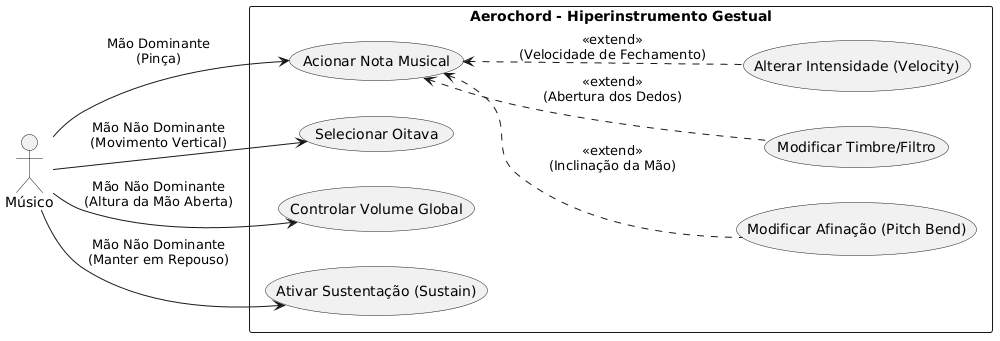
\includegraphics[width=0.85\linewidth]{imagens/casos_uso.png}
    \fonte{O Autor (2026).}
\end{figure}

O sistema prevê os seguintes casos de uso principais, que são acionados simultaneamente dependendo do papel de cada mão (controle ou articulação, atribuído por ordem de entrada em quadro — ver Seção~\ref{sec:captura_deteccao}):
\begin{itemize}
    \item \textbf{Acionar Nota:} O caso de uso central, onde o músico realiza o fechamento dos dedos para engatilhar um evento sonoro.
    \item \textbf{Modular Afinação (\textit{Pitch Bend}):} Ação contínua e simultânea à nota ativada, alterando a altura da nota através da inclinação da mão.
    \item \textbf{Controlar Timbre/Filtro:} Modulação contínua do som utilizando a abertura dos dedos.
    \item \textbf{Controlar Volume e Oitava:} Ações de macrocontrole, operadas pela mão de controle, que configuram a região tonal e a intensidade global do som.
    \item \textbf{Acionar Sustentação (\textit{Sustain}):} Manutenção do som após a liberação do gesto original.
\end{itemize}

\section{Arquitetura do Sistema e Concorrência}
\label{sec:arquitetura_concorrencia}

A arquitetura do Aerochord é composta por cinco módulos principais de processamento, além de um módulo opcional de visualização. Para evitar gargalos e garantir que a lentidão momentânea na inferência de vídeo não bloqueie a emissão de comandos MIDI, cada módulo opera em sua própria linha de execução (\textit{thread}) dedicada.

A comunicação inter-processual é realizada exclusivamente por meio de filas de produtor único e consumidor único (\textit{Single-Producer / Single-Consumer} - SPSC) do tipo livres de bloqueio (\textit{lock-free}). Esta estrutura, implementada por meio de espaços de armazenamento temporário (\textit{buffers}) circulares estáticos e operações atômicas com barreiras de memória rigorosas, elimina a necessidade de mecanismos de exclusão mútua (\textit{mutexes}). Na prática, isso impede que uma \textit{thread} bloqueie a outra (\textit{thread blocking}), garantindo que o fluxo de dados musicais no caminho crítico de execução (\textit{hot path}) ocorra sem interrupções por sincronização, requisito fundamental em sistemas de áudio de baixa latência.

O fluxo contínuo de dados atravessa os seguintes estágios:
\begin{enumerate}
    \item \textbf{Captura:} Obtenção de quadros da câmera.
    \item \textbf{Detecção de Pose:} Extração de coordenadas espaciais das mãos.
    \item \textbf{Análise de Gestos:} Tradução de coordenadas em eventos com significado semântico através de uma Máquina de Estados Finitos (\textit{Finite State Machine} - FSM).
    \item \textbf{Mapeamento:} Conversão de intenções gestuais em comandos musicais brutos.
    \item \textbf{Geração MIDI:} Empacotamento e transmissão de protocolos musicais (MIDI 1.0/2.0).
\end{enumerate}

\section{Captura e Detecção de Pose}
\label{sec:captura_deteccao}

A primeira etapa do \textit{pipeline} é gerenciada pelo módulo de captura (\texttt{CaptureModule}), responsável por interagir diretamente com o equipamento físico (\textit{hardware}) de vídeo. Em ambientes Linux, o módulo utiliza a interface V4L2 (\textit{Video4Linux2}) com mapeamento direto de memória (\textit{memory mapping}) para acessar os \textit{buffers} da câmera, evitando cópias desnecessárias na memória do sistema. 

Na sequência, o módulo de detecção (\texttt{PoseDetectionModule}) consome esses quadros e aciona o rastreador de pontos-chave das mãos (\textit{Hand Landmarker}) do MediaPipe. Este módulo extrai 21 pontos de referência anatômicos (\textit{landmarks}) tridimensionais normalizados para até duas mãos simultaneamente. Para mitigar o \textit{jitter} (pequenas oscilações naturais e ruídos na inferência da rede neural) que poderia resultar em ruído sonoro, o sistema aplica um filtro de Média Móvel Exponencial (EMA) sobre as coordenadas espaciais. Adicionalmente, um algoritmo de correspondência espacial por proximidade do pulso garante que as detecções não troquem de papel inadvertidamente entre os quadros, preservando a coerência da atribuição de cada mão ao longo do tempo.

A atribuição inicial dos papéis de cada mão (controle vs.\ articulação) é feita por \textbf{ordem de entrada em quadro}, e não pela classificação de lateralidade (esquerda/direita) do MediaPipe: a primeira mão detectada após um período sem nenhuma mão em quadro assume o papel de controle (volume/oitava); a segunda mão a entrar assume o papel de articulação (pinça/notas). Essa escolha de projeto decorre da baixa confiabilidade da classificação de lateralidade do MediaPipe quando apenas uma mão está visível, sem o contexto da outra mão para comparação — o que tornaria o rótulo bruto do modelo uma base instável para a divisão de papéis. Como efeito colateral desejável, esse critério torna o sistema utilizável tanto por destros quanto por canhotos sem qualquer configuração: o usuário simplesmente posiciona primeiro a mão que deseja usar para controle.

\section{Máquina de Estados e Análise Gestual}
\label{sec:fsm_analise}

O módulo de análise (\texttt{GestureAnalysisModule}) atua como o motor lógico do sistema. Ele ingere as coordenadas filtradas e extrai métricas geométricas, como distâncias euclidianas e ângulos relativos, alimentando a Máquina de Estados Finitos (FSM) que identifica a intenção musical do usuário.

Visando acessibilidade e ergonomia irrestrita (suportando usuários destros e canhotos sem qualquer configuração prévia), o sistema divide as responsabilidades entre dois papéis funcionais, atribuídos por ordem de entrada em quadro conforme descrito na Seção~\ref{sec:captura_deteccao}:
\begin{itemize}
    \item \textbf{Mão de Articulação e Modulação (segunda a entrar em quadro):} Controla o gatilho das notas através de um gesto de "pinça" (aproximação entre polegar e indicador). A FSM transita pelos estados de inatividade (\texttt{IDLE}), início de pinça (\texttt{PINCH\_START}) e sustentação de pinça (\texttt{PINCH\_HOLD}). Durante a sustentação, o módulo extrai variações contínuas, como o ângulo de inclinação da mão para modulação de afinação (\textit{Pitch Bend}) e a taxa de oscilação lateral para controle de \textit{Vibrato}.
    \item \textbf{Mão de Macrocontrole (primeira a entrar em quadro):} Opera majoritariamente de forma contínua. A altura vertical da mão aberta traduz-se em controle global de volume. Um gesto de pinça acompanhado de movimento vertical aciona a transição de oitavas, enquanto manter a mão em repouso por um período pré-determinado alterna o estado do pedal de sustentação (\textit{Sustain}).
\end{itemize}

Como o papel de cada mão é definido pela ordem de entrada e não pela lateralidade anatômica, o usuário escolhe livremente qual mão (esquerda ou direita) deseja usar para articulação, bastando posicioná-la em quadro depois da mão de controle.

Para garantir estabilidade, o módulo implementa lógicas de estabilização de sinal (\textit{debounce}, exigindo estabilidade por quadros consecutivos) e \textit{histerese} (diferença de limiares) nas transições de estado, prevenindo engatilhamentos duplos e acidentais das notas.

\section{Estratégias de Mapeamento Gesto-Som}
\label{sec:estrategias_mapeamento}

O módulo de mapeamento (\texttt{MappingModule}) consome os eventos gestuais semânticos e os traduz em comandos MIDI, atuando como a interface entre o movimento físico e a teoria musical.

A Tabela~\ref{tab:mapeamento_implementado} descreve o conjunto de mapeamentos implementados, detalhando cada gesto básico, a ação musical correspondente e a justificativa para a escolha do gesto em termos ergonômicos e perceptivos, respeitando a lógica de lateralidade.

\begin{table}[htbp]
    \centering
    \caption{Mapeamento Gesto–Som Implementado no Aerochord}
    \label{tab:mapeamento_implementado}
    {\scriptsize
     \setlength{\tabcolsep}{2pt}
     \renewcommand{\arraystretch}{1.0}
     \begin{tabularx}{\textwidth}{L{2.5cm} L{2cm} L{4.5cm} X}
        \toprule
        \textbf{Função Musical} & \textbf{Mão (ordem de entrada)} & \textbf{Gesto Utilizado} & \textbf{Justificativa} \\
        \midrule
        Seleção de Oitava 
            & 1\textsuperscript{a} (controle)
            & Pinça + movimento vertical. 
            & Gesto modal claro que separa o controle de oitava de outras funções, evitando acionamentos acidentais. \\
        \addlinespace
        Volume Global 
            & 1\textsuperscript{a} (controle)
            & Mão aberta + movimento vertical. 
            & Mapeamento intuitivo (cima/baixo = mais/menos) que utiliza um gesto natural de ``repouso''. \\
        \addlinespace
        Disparo de Nota 
            & 2\textsuperscript{a} (articulação)
            & Pinça (polegar + indicador) em zonas verticais discretas. 
            & Gesto ergonômico e preciso para iniciar o som. A altura da mão define a nota de forma intuitiva. \\
        \addlinespace
        Parada de Nota 
            & 2\textsuperscript{a} (articulação)
            & Soltar o gesto de pinça. 
            & Ação de abrir a mão é a contraparte mecânica e imediata ao gesto de disparo. \\
        \addlinespace
        Timbre/Filtro 
            & 2\textsuperscript{a} (articulação)
            & Distância entre a ponta do dedo médio e a palma. 
            & Gesto robusto para rastreamento que oferece grande amplitude expressiva sem influenciar a afinação. \\
        \addlinespace
        \textit{Pitch Bend} 
            & 2\textsuperscript{a} (articulação)
            & Inclinação (rotação) da mão. 
            & Movimento angular é ortogonal ao movimento de seleção de nota, minimizando conflitos de leitura. \\
        \addlinespace
        \textit{Vibrato} 
            & 2\textsuperscript{a} (articulação)
            & Oscilação leve lateral. 
            & Mimetiza mecanicamente o \textit{vibrato} de instrumentos de corda acústicos. \\
        \addlinespace
        Intensidade (\textit{Velocity}) 
            & 2\textsuperscript{a} (articulação)
            & Velocidade temporal de fechamento da pinça. 
            & Imita a física de instrumentos de percussão e teclas (tocar mais rápido gera um ataque mais intenso). \\
        \bottomrule
     \end{tabularx}
    }
\end{table}

Observa-se que a mão de controle foi minimamente utilizada, o que abre margem para expansões futuras de controle (como acionamento de acordes inteiros ou mudança de programas). O mapeamento discrimina claramente ações discretas (ativação de nota) e modulações contínuas.

O sistema divide a área de atuação da câmera em 12 zonas verticais, correspondentes aos semitons de uma oitava completa. O mapeamento incorpora zonas mortas (\textit{dead zones} — áreas de fronteira sem resposta) e preenchimento (\textit{padding}) nas extremidades superior e inferior do quadro visual. Isso fixa as notas mais graves e agudas, garantindo que o \textit{performer} não precise esticar o braço até os limites físicos do alcance da câmera para tocar as notas extremas da escala.

Um recurso de destaque na implementação é o modo de ligação (\textit{legato}). Quando ativado, o mapeador permite a transição de notas de forma fluida (deslizando a mão de articulação ainda fechada entre as zonas verticais). A engenharia do módulo garante que o comando da nova nota (\texttt{NOTE\_ON}) seja emitido milissegundos antes do encerramento da nota anterior (\texttt{NOTE\_OFF}), criando a sobreposição de áudio necessária para que os sintetizadores engatilhem transições fluídas, mimetizando instrumentos de sopro.

\section{Geração de Protocolo e Suporte Nativo a MIDI 2.0}
\label{sec:geracao_protocolo}

A etapa final reside no módulo de comunicação, responsável por formatar e entregar os comandos musicais ao sistema operacional. O Aerochord inova ao implementar suporte ao padrão MIDI 2.0 através da formatação de Pacotes MIDI Universais (\textit{Universal MIDI Packet} - UMP).

Durante a inicialização, o sistema executa um processo de negociação inicial (\textit{handshake}) via Consulta de Capacidades (\textit{Capability Inquiry} - MIDI-CI), enviando mensagens de descoberta (\textit{Discovery}) para verificar se o dispositivo receptor suporta a nova especificação. Sendo compatível, o sistema constrói pacotes UMP de 64 bits e os despacha. Isso garante resoluções de 32 bits para mensagens de controle contínuo, além de permitir o \textit{Per-Note Pitch Bend} (dobra de afinação individualizada por nota ativa), elevando drasticamente o teto de expressividade instrumental da aplicação.

Caso o equipamento ou \textit{software} receptor não suporte o novo padrão, o sistema aplica um mecanismo de contingência (\textit{fallback}) transparente, truncando matematicamente os dados para os 7 bits originais e roteando a comunicação via arquitetura legado (MIDI 1.0), assegurando total compatibilidade com tecnologias anteriores e garantindo a universalidade da solução.
\chapter{Testes e Análise de Resultados}
\label{chap:testes_resultados}

Após o desenvolvimento e a implementação da arquitetura do Aerochord, tornou-se imperativo submeter o sistema a um processo de validação empírica. Este capítulo detalha os testes realizados para aferir se a ferramenta atingiu as metas propostas nos requisitos não funcionais e funcionais.

A avaliação foi dividida em três frentes complementares. Na Seção~\ref{sec:avaliacao_desempenho}, analisam-se os dados objetivos de desempenho do sistema operando em tempo real, com foco na medição estatística da latência de ponta a ponta (\textit{end-to-end}) e no consumo de recursos da máquina. Na Seção~\ref{sec:avaliacao_qualitativa}, discute-se a estabilidade do rastreamento gestual e a qualidade percebida das articulações e mapeamentos. Por fim, na Seção~\ref{sec:teste_usabilidade}, apresenta-se um teste piloto de usabilidade conduzido com um voluntário, visando validar a acessibilidade técnica e a curva de aprendizagem do hiperinstrumento.

\section{Avaliação de Desempenho Técnico e Latência}
\label{sec:avaliacao_desempenho}

O requisito técnico mais crítico para qualquer Instrumento Musical Digital é a manutenção de uma latência imperceptível para o intérprete, garantindo a sensação de causalidade imediata entre o gesto físico e o evento sonoro. A literatura estabelece que latências de ponta a ponta abaixo de 30 milissegundos (ms) são consideradas ideais para preservar a tocabilidade em interfaces musicais interativas.

Para medir essa métrica, o Aerochord foi executado em um computador pessoal, equipado com sistema operativo Linux, utilizando o modo analítico (\texttt{--eval}). Neste modo, o \textit{software} regista marcações temporais (\textit{timestamps}) exatas no momento em que um quadro de vídeo é capturado pelo software (entregue pelo subsistema de vídeo) e, em seguida, regista o momento exato em que a mensagem MIDI 2.0 correspondente é enviada para o sequenciador do sistema operacional. Cabe ressaltar que essa métrica isola a latência do \textit{pipeline} de \textit{software} — da captura do quadro ao envio da mensagem MIDI —, não incluindo a latência intrínseca da câmera (exposição do sensor e transferência de dados) nem a renderização de áudio do sintetizador receptor, ambas independentes da implementação.

O teste de carga contínua consistiu na execução da aplicação por um período prolongado de interação ativa, gerando um conjunto de dados (\textit{dataset}) com 7.821 amostras de eventos musicais consecutivos.

\subsection{Resultados de Latência}
A análise estatística do arquivo de registo gerado pelo sistema demonstrou resultados altamente satisfatórios, superando a meta estabelecida. Os dados recolhidos foram:
\begin{itemize}
    \item \textbf{Amostras totais:} 7.821 eventos.
    \item \textbf{Latência Média:} 22,62 ms.
    \item \textbf{Percentil 50 (P50 - Mediana):} 22,29 ms.
    \item \textbf{Percentil 95 (P95):} 24,73 ms.
    \item \textbf{Amostras abaixo de 30 ms:} 99,2\%.
\end{itemize}

O indicador P95 de 24,73 ms atesta que 95\% de todos os eventos musicais gerados pelo sistema — desde a captura do quadro pelo software até o envio da mensagem MIDI — ocorreram em menos de 24,8 milissegundos. Este valor, associado a uma taxa de sucesso de 99,2\% das amostras abaixo da tolerância máxima de 30 ms, prova a eficácia da arquitetura concorrente baseada em filas livres de bloqueio (\textit{lock-free}) implementada em C++.

\subsection{Consumo de Recursos do Sistema}
O desempenho de baixa latência seria inviável se o consumo de recursos computacionais saturasse o sistema operacional, resultando no descarte de quadros (\textit{frame drops}). Durante os testes em tempo real, a aplicação consumiu em média \textbf{25,27\% de CPU} (medida em relação à capacidade total da máquina) e utilizou \textbf{145,0 MB de Memória RAM}, considerando o \textit{pipeline} central de processamento (captura, detecção, análise, mapeamento e geração MIDI), sem a janela de visualização opcional.

Estes números demonstram que a integração da biblioteca MediaPipe nativa em C++ oferece um impacto computacional significativamente leve. O sistema preserva recursos suficientes para que o mesmo computador possa, simultaneamente, executar uma Estação de Trabalho de Áudio Digital (DAW) e processar sintetizadores virtuais pesados, cumprindo na íntegra a premissa de acessibilidade de \textit{hardware}.

\subsection{Distribuição e Expressividade dos Eventos}
A análise do \textit{dataset} de 7.821 amostras também revelou a distribuição por tipo de mensagem MIDI gerada durante a execução:
\begin{itemize}
    \item \textbf{Eventos de Nota (\textit{Note On / Note Off}):} 822 amostras (10,5\%).
    \item \textbf{Controladores Contínuos (\textit{Control Change} - CC):} 4.805 amostras (61,4\%).
    \item \textbf{Dobra de Afinação por Nota (\textit{Per-Note Pitch Bend}):} 2.194 amostras (28,1\%).
\end{itemize}

Este perfil de distribuição, onde aproximadamente 89,5\% das mensagens consistem em dados de modulação contínua (CC e Afinação), evidencia matematicamente a filosofia de \textit{design} focada no movimento (\textit{movement-first}). O Aerochord não funciona como um mero disparador de notas estáticas; a maioria dos dados processados reflete a expressividade contínua do corpo do intérprete moldando o som no decurso do tempo.

\section{Estabilidade e Avaliação Qualitativa}
\label{sec:avaliacao_qualitativa}

Além dos dados quantitativos, uma avaliação qualitativa do uso prolongado permitiu inferir a estabilidade e a ergonomia do instrumento sob condições reais.

Observou-se que a detecção do gesto de "pinça" (gatilho de nota da mão de articulação) obteve uma taxa de precisão qualitativa de aproximadamente 90\%. As falsas detecções (falsos positivos ou negativos) mostraram-se residuais e estão diretamente ligadas a condições do ambiente externo, nomeadamente ao enquadramento excessivamente descentrado da mão ou a condições de iluminação desfavoráveis, fatores inerentes a abordagens por visão monocular. Em condições de iluminação estável, o sistema mostrou-se altamente responsivo.

O modo de transição fluida de notas (\textit{legato}), suportado pela sobreposição temporal de eventos através do algoritmo de programação, desempenhou a sua função de maneira satisfatória, assegurando transições limpas. Foram registadas falhas esporádicas no acoplamento das notas apenas em ocasiões onde os movimentos do utilizador excederam o limiar de tolerância algorítmico nas zonas de fronteira (zonas mortas).

Quanto à divisão de papéis entre as mãos, a alocação dos macro-controles (seleção de oitavas e volume) para a \textbf{mão de controle} (a primeira a entrar em quadro) revelou-se natural. Constatou-se, contudo, que tocar articulações com a mão de articulação enquanto se realizam saltos simultâneos de oitava com a mão de controle exige coordenação e prática prévia por parte do executante. Por outro lado, performances confinadas a uma única oitava, utilizando ambas as mãos predominantemente para timbre e intensidade, demonstraram uma fluidez e curva de aprendizagem bastante acessíveis.

\section{Teste Piloto de Usabilidade: Estudo de Caso}
\label{sec:teste_usabilidade}

A fim de verificar a facilidade de uso e avaliar o baixo custo de entrada (que preconiza a utilização da interface por indivíduos sem formação musical), realizou-se um teste piloto empírico de usabilidade.

O voluntário, designado como Participante 1 (P1), encaixa-se no perfil-alvo de acessibilidade: não possui treino musical formal nem contato rotineiro com instrumentos acústicos tradicionais, embora revele um interesse passivo por música. 

\subsection{Metodologia do Teste e Curva de Aprendizagem}
O teste foi conduzido num ambiente não controlado (doméstico). Foi fornecida a P1 uma breve instrução verbal, com duração inferior a 5 minutos, explicando a separação funcional de papéis entre as mãos (a mão de articulação executa notas e a mão de controle controla a região das oitavas e o volume), atribuídos automaticamente pela ordem de entrada em quadro. 

Após a explicação inicial, P1 iniciou a exploração livre do hiperinstrumento. Sem qualquer necessidade de intervenção do investigador ou consulta a diagramas, o participante foi capaz de gerar sequências melódicas intencionais, controlando o volume e transitando entre oitavas logo nos primeiros minutos de utilização. O sucesso imediato de P1 em operar o Aerochord, em contraste direto com a longa curva de aprendizagem requerida por instrumentos de cordas ou sopro convencionais, suporta empiricamente a hipótese de que o sistema possui uma barreira técnica de entrada extremamente baixa.

\subsection{Feedback Qualitativo e Limitações Identificadas}
Após a sessão exploratória, o participante forneceu suas impressões verbais sobre a experiência (retorno sensorial / \textit{feedback} qualitativo). O sistema foi descrito como altamente reativo e de fácil compreensão mecânica.

Entretanto, durante o relato final, P1 fez a seguinte observação crucial sobre a profundidade funcional da aplicação:
\begin{quote}
"Hoje vejo que só é possível tocar notas soltas no software. Seria interessante poder tocar acordes."
\end{quote}

Este apontamento evidencia não apenas a assimilação rápida do funcionamento da ferramenta por parte do participante, mas também identifica uma limitação funcional arquitetônica da versão atual do Aerochord: o mapeamento de um único rastreador de pinça por mão restringe a execução à monofonia ou a melodias de nota única. O desejo orgânico do utilizador de expandir o escopo sonoro para execuções harmônicas completas (acordes polifônicos) será discutido como o principal foco de trabalho futuro do sistema.
\chapter{Considerações Finais}
\label{chap:consideracoes_finais}

Este trabalho propôs o desenvolvimento e a avaliação do Aerochord, um hiperinstrumento musical gestual fundamentado em visão computacional e no protocolo MIDI 2.0. A motivação central da pesquisa originou-se na observação de uma lacuna significativa no estado da arte: a ausência de sistemas que aliassem acessibilidade — dispensando equipamentos físicos (\textit{hardware}) de alto custo —, baixa latência e expressividade de nível profissional. Ao longo dos capítulos, a transição da fundamentação teórica para a implementação prática demonstrou que é possível democratizar a execução musical sem abdicar do rigor técnico.

A pesquisa cumpriu os seus objetivos delineados no Capítulo~\ref{chap:introducao}. A revisão bibliográfica consolidou o entendimento sobre a interação humano-computador aplicada à música e a evolução dos hiperinstrumentos. A adoção do protocolo MIDI 2.0 provou ser um diferencial crítico: a modulação de alta resolução (controle contínuo de 32 bits e \textit{velocity} de 16 bits) eliminou os saltos audíveis do padrão legado, conferindo resposta sonora refinada já na versão atual. Adicionalmente, o sistema emprega a dobra de afinação por nota individual (\textit{Per-Note Pitch Bend}) — recurso inexistente no MIDI 1.0 — que, embora na versão monofônica atual seja equivalente em efeito audível à dobra por canal, prepara a arquitetura para a expressividade polifônica prevista nos trabalhos futuros. A arquitetura dos programas de computador (\textit{software}), construída em linguagem C++ e utilizando o arcabouço (\textit{framework}) JUCE em conjunto com a biblioteca MediaPipe, materializou esses conceitos numa solução robusta e funcional.

\section{Síntese dos Resultados}
\label{sec:sintese_resultados}

A avaliação empírica do Aerochord comprovou a viabilidade técnica e prática da proposta. Em termos de desempenho, a arquitetura baseada em esteiras de processamento assíncronas (\textit{pipelines}) e filas livres de bloqueio (\textit{lock-free}) foi capaz de manter a latência de ponta a ponta (\textit{end-to-end}) rigorosamente controlada. O percentil 95 (P95) de 24,73 milissegundos atesta que o sistema opera consistentemente abaixo da barreira perceptível de 30 milissegundos, um marco notável para uma aplicação que realiza inferência de redes neurais em tempo real sobre imagens de vídeo. 

Simultaneamente, o consumo de recursos da máquina revelou-se altamente eficiente (consumindo cerca de 25\% de CPU e aproximadamente 145 MB de memória RAM num ambiente de teste padrão), confirmando a sustentabilidade da execução do Aerochord em paralelo com Estações de Trabalho de Áudio Digital (DAWs) num mesmo computador de uso doméstico. 

Na perspectiva da usabilidade, o teste piloto empírico demonstrou que o hiperinstrumento possui uma barreira técnica de entrada muito baixa. O modelo de interação centrado na distinção ergonômica entre a mão de articulação (para notas e efeitos) e a mão de controle (para macro-controles como volume e oitavas), com os papéis atribuídos pela ordem de entrada em quadro, mostrou-se natural. Essa separação de papéis permitiu que um performador sem formação musical formal compreendesse o sistema e gerasse melodias expressivas com menos de cinco minutos de instrução preliminar.

\section{Limitações do Estudo}
\label{sec:limitacoes}

Apesar dos resultados positivos, o sistema apresenta limitações inerentes à tecnologia escolhida e às decisões iniciais de projeto (\textit{design}). A utilização de visão monocular (captura por uma única lente de \textit{webcam}) torna a aplicação dependente de boas condições de iluminação e de um enquadramento visual claro. Situações de oclusão mecânica das mãos ou movimentos excessivamente rápidos que gerem borrão de movimento (\textit{motion blur}) podem induzir falhas pontuais no rastreamento dos pontos de referência anatômicos (\textit{landmarks}).

Adicionalmente, a lógica de acionamento musical desenvolvida na versão atual da Máquina de Estados Finitos restringe a execução a uma única nota por vez na mão de articulação (monofonia). O mapeamento de um único gesto de pinça global impede, momentaneamente, a formulação de blocos harmônicos simultâneos no mesmo canal.

\section{Trabalhos Futuros}
\label{sec:trabalhos_futuros}

As limitações identificadas e o retorno avaliativo (\textit{feedback}) qualitativo obtido durante os testes abrem um leque de oportunidades promissoras para a continuidade deste trabalho. Entre as principais diretrizes para evolução do Aerochord, destacam-se:

\begin{itemize}
    \item \textbf{Implementação de Polifonia e Acordes:} Conforme apontado diretamente pelo participante do teste piloto empírico (que expressou o forte desejo de tocar acordes em vez de notas soltas), o desenvolvimento de uma lógica para reconhecer o fechamento independente de múltiplos dedos permitirá a execução de harmonias completas, elevando o nível de virtuosidade da aplicação.
    \item \textbf{Mapeamentos Inteligentes via Aprendizado de Máquina (\textit{Machine Learning}):} Integrar algoritmos que aprendam o vocabulário gestual individual do intérprete, ajustando automaticamente as curvas de sensibilidade e as zonas mortas (\textit{dead zones}) em tempo real, personalizando ainda mais a experiência ergonômica.
    \item \textbf{Fusão Multimodal:} Combinar o rastreamento da \textit{webcam} com Unidades de Medição Inercial presentes em dispositivos vestíveis comuns, como relógios inteligentes (\textit{smartwatches}), para mitigar as falhas de oclusão visual da lente monocular e aumentar a precisão dos gestos.
    \item \textbf{Exploração em Ambientes Imersivos:} Expandir a saída de dados do sistema para controlar motores (\textit{engines}) sonoros em ambientes de Realidade Virtual e Realidade Aumentada (VR/AR), tirando proveito da arquitetura assíncrona de baixa latência já estabelecida.
\end{itemize}

Em suma, o Aerochord consolida-se como um passo significativo em direção à democratização da musicalidade mediada por computador. O equilíbrio alcançado entre o baixo custo estrutural, o alto desempenho computacional e a inovação tecnológica conferida pelo protocolo MIDI 2.0 prova que a expressão musical gestual digital não precisa ser um privilégio exclusivo de laboratórios e estúdios avançados, podendo ser acessível, responsiva e profundamente expressiva para qualquer pessoa com um computador e uma câmera.
%\include{2-textuais/nomedoarquivo sem .tex}

%=======================================================================
% ELEMENTOS PÓS-TEXTUAIS
%=======================================================================
\postextual

% ----------------------------------------------------------------------
% Referências bibliográficas
% ----------------------------------------------------------------------
\bibliographystyle{abntex2-alf}
\bibliography{3-pos-textuais/referencias.bib}

% ----------------------------------------------------------------------
% Apêndices (se necessário)
% ----------------------------------------------------------------------
%\include{3-pos-textuais/apendices}

% ----------------------------------------------------------------------
% Anexos (se necessário)
% ----------------------------------------------------------------------
%\include{3-pos-textuais/anexos}

\end{document}